\documentclass[12pt]{article}
\usepackage{enumitem}
%\usepackage[T1]{fontenc}
\usepackage[auth-sc,affil-sl]{authblk}
\usepackage{amsmath}
\usepackage{graphicx}
\usepackage{color}
\usepackage[toc,page]{appendix}
%\usepackage{enumerate}
\usepackage[round]{natbib}
%\usepackage{url} % not crucial - just used below for the URL 
%\usepackage{amsthm}
\usepackage{amssymb}
\usepackage{graphicx}
\usepackage{epstopdf}
\usepackage{hyperref}
\usepackage{alltt}
\usepackage{listings}
\usepackage{array}
\usepackage[noline, boxed, linesnumbered, procnumbered, titlenumbered]{algorithm2e}
%\usepackage[firstpage]{draftwatermark}
\usepackage[margin=1in]{geometry}  %%jcgs has own margins
\usepackage{lmodern}
\usepackage{caption}
\usepackage{subcaption}

%\pdfminorversion=4
% NOTE: To produce blinded version, replace "0" with "1" below.
\newcommand{\blind}{0}

\newcommand{\secref}[1]{Section~\ref{#1}}
\newcommand{\appdxref}[1]{Appendix~\ref{#1}}
\newcommand{\tblref}[1]{Table~\ref{#1}}
\newcommand{\figref}[1]{Figure~\ref{#1}}
\newcommand{\thmref}[1]{Theorem~\ref{#1}}
\newcommand{\algref}[1]{Algorithm~\ref{#1}}
\newcommand{\funref}[1]{Function~\ref{#1}}
\newcommand{\listingref}[1]{Listing~\ref{#1}}

\newcommand{\eg}{{\em e.g.}}
\newcommand{\ith}{$i^{th}$}
\newcommand{\cut}[1]{}
\newcommand{\todo}[1]{{{\color{red}{[#1]}}}}

\newcommand{\spd}{\fontfamily{cmr}\textsc{\small StratPD}}
\newcommand{\cspd}{\fontfamily{cmr}\textsc{\small CatStratPD}}
\newcommand{\xnc}{$x_{\overline{c}}$}
\newcommand{\xnC}{$x_{\overline{C}}$}

\setlist[enumerate]{itemsep=-1mm}

% DON'T change margins - should be 1 inch all around.
\cut{
\addtolength{\oddsidemargin}{-.5in}%
\addtolength{\evensidemargin}{-.5in}%
\addtolength{\textwidth}{1in}%
\addtolength{\textheight}{1.3in}%
\addtolength{\topmargin}{-.8in}%
}

\begin{document}

\def\spacingset#1{\renewcommand{\baselinestretch}%
{#1}\small\normalsize} \spacingset{1}


%%%%%%%%%%%%%%%%%%%%%%%%%%%%%%%%%%%%%%%%%%%%%%%%%%%%%%%%%%%%%%%%%%%%%%%%%%%%%%

\if0\blind
{
  \title{\bf A Stratification Approach to Partial Dependence for Codependent Variables}

  \author{Terence Parr and James D. Wilson\\
      University of San Francisco\\
}
  \maketitle
} \fi

\if1\blind
{
  \bigskip
  \bigskip
  \bigskip
  \begin{center}
    {\LARGE\bf Title}
\end{center}
  \medskip
} \fi

\bigskip
\begin{abstract}
Interpretability is becoming increasingly important to machine learning practitioners, and a key component of  interpretation is the characterization of partial dependence of the response variable on any subset of features used in the model. The two most common strategies for assessing partial dependence---linear regression and partial dependence plots---suffer from a number of critical weaknesses. In the first strategy, linear regression model coefficients describe how a unit change in an explanatory variable changes the response, while holding other variables constant. But, linear regression is inapplicable for high dimensional ($p>n$) data sets and is often insufficient to capture the relationship between explanatory variables and the response.  In the second strategy, Partial Dependence (PD) plots and Individual Conditional Expectation (ICE) plots give biased results for the common situation of codependent variables and they rely on fitted models provided by the user. When the supplied model is a poor choice due to systematic bias or overfitting, PD/ICE plots provide little (if any) useful information. To address these issues, we introduce a new strategy, called \spd{}, that (i) does not depend on a user's fitted model, (ii) provides accurate results in the presence of codependent variables, and (iii) is applicable to high dimensional settings. \spd{} is a stratification method that first partitions an observed data set into groups of observations that are similar, except in the variable of interest, through the use of a decision tree and next applies a simple local linear regression on the variable of interest for each group. The resulting partial dependence on a variable is assessed using these local linear coefficients. We apply \spd{} to a collection of simulations and case studies to show that \spd{} is a fast, reliable, and robust method for assessing partial dependence with clear advantages over state-of-the-art methods. 
\end{abstract}

\noindent%
{\it Keywords:} partial dependence, model interpretability, random forests, linear models
%\vfill

%\newpage
%\spacingset{1.5} % DON'T change the spacing!
\section{Introduction}
\label{sec:intro}

%Adding more context and references to our problem -JW (History)
When choosing a supervised model that relates feature and response pairs, model interpretability is often at odds with predictive power. Indeed, these two objectives have traditionally led to the choice of either an interpretable \emph{or} a predictive model (see for example \cite{shmueli2010explain}). This choice has largely been dictated by machine learning and statistics cultures \citep{breiman2001statistical, donoho201750}, where machine learning practitioners focus on predictive ability and statistical practitioners focus on interpretability and inference. Recently, however, there has been a shift in the division of these two objectives as the machine learning community has begun to build what are being called  ``interpretable machine learning'' models \citep{doshi2017towards, vellido2012making}. Interpretable machine learning models aim to get the best of both worlds by achieving high predictive power and ensuring that the predictions of the model can be easily interpreted. 

%importance
In practice machine learning model interpretation is just as important as, and in many cases more important than, obtaining a highly predictive model. Interpretable models play an essential role in artificial intelligence \citep{adadi2018peeking}, where the interpretation of models with high predictive power like neural networks and deep learning techniques are essential to ensure robust, replicable outcomes. Interpretable models are also at the heart of applications in medicine such as precision medicine as well as psychology and psychiatry, where models are used to describe the relationship between an individual's demographic and clinical features and their susceptibility to illness and disease, among other measureable outcomes \citep{dwyer2018machine, katuwal2016machine}.

A key component of model interpretation involves the characterization of the partial dependence of the response on any subset of the features used in the model. For example, consider the aforementioned example of precision medicine. The success of a prevention plan for a ``high-risk" individual depends on their disease susceptibility as well as their clinical characteristics (e.g., age and co-morbidities). That is, the effect that these characteristics have on the person's susceptibility guides the development of a prevention plan and often times is more important than the accuracy of predicting one's chances of the disease itself. 

To describe partial dependence more formally, suppose that $\mathbf{X}$ is an $n \times p$ matrix whose $p$ columns represent observed features, and $\mathbf{y}$ is $n \times 1$ vector of responses. Supervised algorithms seek the unknown model $f:\mathbb{R}^{n \times p} \rightarrow \mathbb{R}^n$ that describes the relationship between $\mathbf{X}$ and $\mathbf{y}$ as $\mathbf{y} = f(\mathbf{X}).$ Let $C \subset \{1, \ldots, p\}$ denote the index set of a subset of features and let $\mathbf{X}_C$ denote the $n \times |C|$ submatrix corresponding to these features. Assessing the partial dependence of $\mathbf{y}$ on features $\mathbf{X}_C$, can be viewed as estimating the unknown function $f_C: \mathbb{R}^{n \times p} \rightarrow \mathbb{R}^n$ that best characterizes the dependence of $\mathbf{y}$ on $\mathbf{X}_C$ given $\mathbf{X}$:

\begin{equation}\label{problem}
	\mathbf{y} = f_C(\mathbf{X}).
\end{equation}


There are a number of strategies for assessing partial dependence, which we describe in detail in Section 1.1. As we'll demonstrate, these methods generally suffer from one or more the following issues:

\begin{itemize}
	\item[(i)] {\bf Model dependence:} Partial dependence depends on a fitted model for $f$, $\widehat{f}$. Thus the accuracy of such methods rely on the accuracy (and sensibility) of the chosen machine learning model. Indeed, model dependent methods for partial dependence focus on the relationship between model \emph{prediction} and features rather than the \emph{response} and the features. This is problematic for several reasons. First, $\widehat{f}$ may not be a reliable model and could, for instance, sacrifice local accuracy to minimize some global loss function. Indeed, in the case that the fitted model is a poor choice, partial dependence does not provide any useful information for the user. Furthermore, different models fitted to the same data can look very different, making the partial dependence of $y$ on $X_C$ unclear.
	\item[(ii)] {\bf Variable codependence:} Partial dependence requires that the features in $\mathbf{X}$ be pairwise independent. In practice this is rarely the case and so results from PD and ICE can lead to improper interpretations because the potentially inaccurate model feeds off of potentially-nonsensical, synthesized observations arising from variable codependencies. 
	\item[(iii)] {\bf Curse of dimensionality:} Partial dependence requires $X$ to be low-dimensional ($n >> p$) and misleading information and biases are introduced when $p > n$. 
\end{itemize}

In light of these challenges, the goal of this work is to characterize partial dependence in a way that (i) does not rely on, nor make predictions from, a user's model,  (ii) does not presume mutually-independent features, and (iii) can be generally applied in high-dimensional settings. We introduce a strategy, called {\textsc{strat}ified \textsc{p}artial \textsc{d}ependence} (\spd{}), that directly estimates the partial dependence of each feature without the need of a fitted model. \spd{} first stratifies the feature space of $\mathbf{X}$ into disjoint regions of observations so that all variables \xnC{}, where $\overline{C} = \{1, \ldots, p\} \setminus C$, are approximately matched across the observations in that region. The relationship between $y$ and $X_C$ in each region is characterized by binning ${x}_C$ itself into disjoint regions and fitting a local linear approximation through each region. We describe \spd{} for numerical explanatory variables in \secref{sec:numerical} and categorical variables in \secref{appendix:catstrat}. We apply our approach to a testbed of simulations and case studies in \secref{sec:applications}, finding that \spd{} provides a fast, reliable, and robust method for assessing partial dependence even in the presence of codependencies. 

\subsection{Existing Methods for Partial Dependence}

Given a model $y = f(X)$, partial dependence methods seek to identify a function $f_C(\cdot)$ that characterizes the partial dependence of a subset of variables $X_C$, as in (\ref{problem}). When $X$ contains only one feature, a plot of the response against the feature can be used to visualize the marginal effect of the feature exactly. Given two or more features, one can similarly plot the marginal effects of each feature separately; however, the analysis is complicated by the interactions of the variables. Generally, pairwise interaction plots are used to visualize interactions between each pair of variables; however, these are limited to pairwise analyses since interaction plots cannot directly visualize interactions along more than three dimensions \citep{cox2014multivariate}.

To circumvent this limitation, traditional marginal plots project other axes onto the plane associated with the feature of interest and target variable. This results in marginal plots that do not isolate the specific contribution of a feature of interest to the target. For example, a marginal plot of sex (male/female) against body weight would likely show that, on average, men are heavier than women. While true, men are also taller than women on average, which likely accounts for most of the difference in average weight. It's unlikely that two ``identical'' people, differing only in sex, would be appreciably different in weight.  

Alternatively, a linear regression model of $y$ on the columns of $\mathbf{X}$ provides the general trend of a single feature $x_c$, $c \in \{1, \ldots, p\}$, on the expected value of $y$ via the estimated regression coefficient $\widehat{\beta}_c$.  For a unit change in $x_c$, the expected value of $y$ increases or decreases by $\widehat{\beta}_c$ while holding all other variables, \xnc{},  fixed.  The major issue with fitting a linear model over the entire domain of $x_c$ lies in the fact it does not capture non-linear relationships between $(X,y)$ observation pairs. This is because the coefficient $\widehat{\beta}_c$ is a constant, which smooths over any local $y$ fluctuations across the entire range of $x_c$.  Also, linear regression models are inapplicable for high dimensional ($p > n$) data sets.

Varying-coefficient models like those introduced in \citet{fan2008statistical} as well as local nonparametric methods like LOESS \citep{cleveland1979robust, cleveland1981lowess, cleveland1988locally} can model effect heterogeneities across the range of $x_c$; however, the partial dependence between $y$ and $x_c$ can be difficult to interpret with these models, and these approaches are not appropriate in high dimensional settings. 

The most widely used strategy to analyze partial dependence involves the combined application of partial dependence (PD) plots \citep{PDP} and individual conditional expectation (ICE) plots \citep{ICE}. PD and ICE both rely on the user first fitting a joint model $\widehat{f}$ for the relationship between $X$ and $y$ and subsequently estimate $f_C$ through analyzing the effect that $X_C$ has on the prediction $\widehat{f}$. PD describes the average marginal effect of $X_C$, while ICE plots describe the dependence of $\widehat{f}$ on $X_C$. PD estimates the partial dependence function using $\widehat{f}^{PD}_C(x_C)$:

\begin{equation*}\label{eq:PD} \widehat{f}^{PD}_C(x_C): = \mathbb{E}_{\overline{C}}\left[\widehat{f}({X})\right] = \int \widehat{f}({X}) d\mathbb{P}(X_{\overline{C}}).\end{equation*}

\noindent The function $\widehat{f}_C(x_C)$ describes the average marginal effect that the features $X_C$ has on the prediction $\widehat{f}$. The partial dependence of $X_C$ is a global representation of variable dependence and averages over any heterogeneous relationships between $\mathbf{y}$ and $x_C$. 

The individual conditional expectation (ICE) plot from \cite{ICE} is a local method which estimates the partial dependence of the prediction $\widehat{f}({X})$ on $x_C$ across individual observations. Suppose that $(X_{i, C}, X_{i, \overline{C}})$ are the values of the $i$th row of $\mathbf{X}$. For each $i$, the ICE plot produces a curve from the fitted model over all values of $X_C$ while holding $X_{i, \overline{C}}$ fixed.  In particular, for observation $i$ the the curve $\widehat{f}((\{X_{i, C}\}_{i = 1}^n, X_{i, \overline{C}}))$. Unlike PD, ICE can identify heterogeneous relationships between the fitted model and the features of interest, $X_C$. By construction, the PD curve for variables $X_C$ is the average over all ICE curves for those variables. In practice, typically both ICE and PD are used to describe the partial dependence of $\mathbf{y}$ on $X_C$.

An important limitation of PD and ICE is that they require independence of the features in $\mathbf{X}$. This is rarely the case in practice, and in such situations these plots lead to faulty inference and misinterpretation (see \cite{apley2016visualizing} for a discussion). \cite{apley2016visualizing} introduced the accumulated local effects (ALE) strategy to overcome the independence limitation. The ALE plot is an average partial dependence of $\widehat{f}$ on $X_C$ that is calculated through the accumulation of local changes in the prediction for small windows of $X_C$. Local changes are measured as gradients of $\widehat{f}$ with respect to $X_C$ while $X_{\overline{C}}$ is held fixed. Although the ALE plot is unbiased in the presence of codependent features, it still has some disadvantages. Unlike \spd{}, ALE is not directly suitable for categorical variables as an ordering of each variable is needed for the calculation of gradients of $\widehat{f}$. Furthermore, the user must determine the number of intervals to use for calculating an ALE plot, and there is no general advice on how to do this.

%LIME
\cite{ribeiro2016should} proposed the local interpretable model-agnostic explanations (LIME) method as a strategy to interpret machine learning predictions. For a prediction of interest, LIME learns an interpretable model, on a small neighborhood of data around that prediction that explains the relationship between variables and the response locally. In contrast to \spd{}, LIME is used to create local interpretable models for each prediction; however, it does not directly assess the partial dependence of the response on a subset of variables. Like LIME, \spd{} also relies upon local interpretable models; however, \spd{} does this to explain partial dependence relationships rather than correlative relationships between the response and features. 

%Shapley
The Shapley strategy, introduced in \cite{lundberg2016unexpected}, is a permutation-based method for estimating the relationship between ${y}$ and the variables $X_C$ through a fitted model $\widehat{f}$. In this method, the marginal effect of $X_C$ is represented by the Shapely value, which is the average change in the prediction made from the original data $\widehat{f}$ and the prediction made when all other variables $X_{\overline{C}}$ have been randomly shuffled in the dataset. The permuting of $X_{\overline{C}}$ is repeated many times and the average Shapely value is reported as the importance. Like PD, ICE, and ALE, the Shapely strategy is also dependent on the machine learning model fitted. Further, like any permutation method, this strategy can suffer from nonsensical observations due to the permuting of $X_{\overline{C}}$, which are subsequently incorporated in the estimated dependence. This is especially problematic in the case of highly-correlated features. Finally, a major disadvantage of the Shapely strategy is its computational complexity due to repeated permutations. 


\section{Motivating Examples}\label{sec:motivation}
We begin by considering two examples that illustrate the possible issues that can arise when using the existing partial dependence strategies outlined in Section 1.1. We focus on the PD and ICE plots, but note that the other mentioned methods face similar challenges. 


\subsection{Model Dependence}
Consider the New York City apartment rent data set from Kaggle \cite{rent} and the marginal plot in \figref{fig:baths_price}(a) showing the number of bedrooms versus price. \figref{fig:baths_price}(b) shows the (zero-centered) PD plot of rent price on the number of bedrooms as a black line. The partial dependence line is the average of the blue lines, which represent the individual conditional expectation (ICE) plots of \cite{ICE}. In this case, the ICE lines depict the model prediction contributions for a single observation as the bedrooms feature shifts through all possible number of bedrooms. Because PD plots represent an average across observations, they can hide a great deal of variability, so it is helpful to combine PD and ICE plots.

\begin{figure}[htbp]
\begin{center}
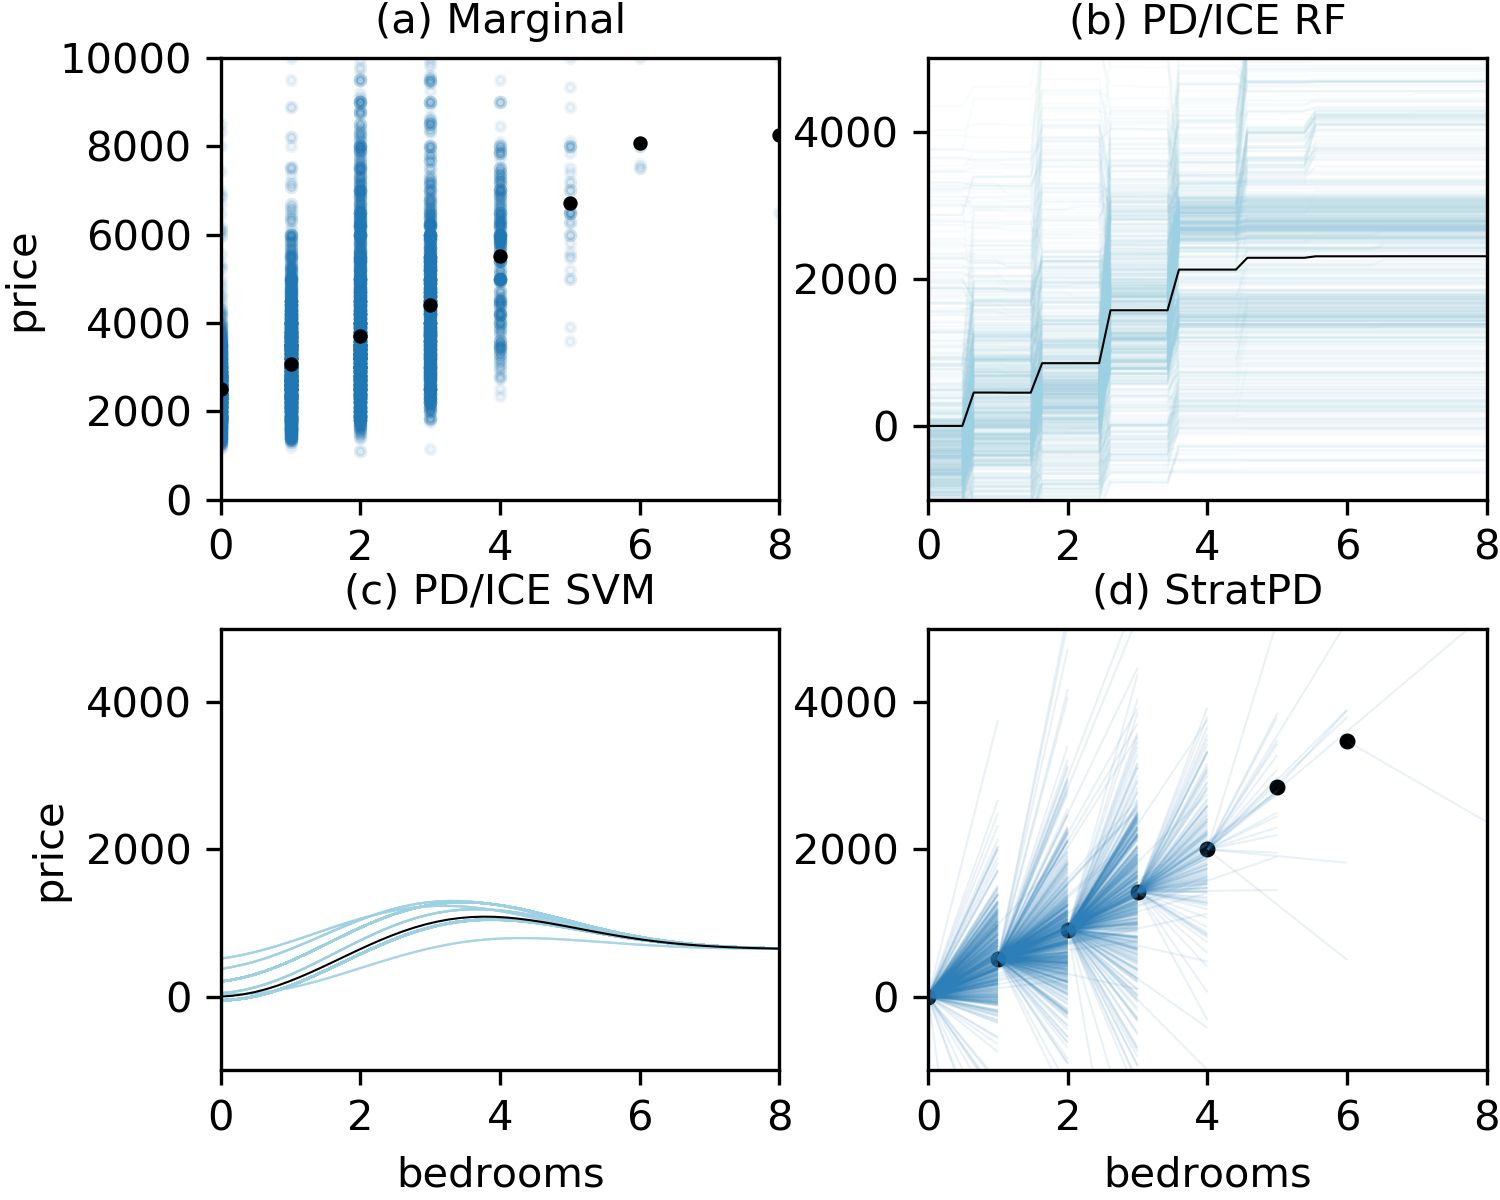
\includegraphics[scale=0.7]{images/bedrooms_vs_price.png}
\caption{Plots of bedrooms versus rent price using New York City apartment rent data. (a) marginal plot, (b) PD/ICE plot derived from random forest, (c) PD/ICE plot derived from SVM, and (d) \spd{} plot; sample size is 10,000 observations of \textasciitilde400k. The PD/ICE plots are radically different for the same data set, depending on the chosen user model.}
\label{fig:baths_price}
\end{center}
\end{figure}

While PD and ICE plots are {\em model-agnostic}, they are not {\em model-independent} and are subject to the strengths and weaknesses of the model making predictions. For example, as seen in \figref{fig:baths_price}(b), random forests (RF) do not well extrapolate beyond their training set support range and this data set subset of 10,000 observations has very few apartments with more than 5 bedrooms. (Note the lack of blue dots in that range of the marginal plot.) PD and ICE plots shift the bedrooms feature of all observations from 0 to 8, accepting less trustworthy predictions from the model in extreme ranges.   

Obtaining radically different PD and ICE plots for different underlying models is undesirable because users cannot distinguish between interesting target fluctuations and artifacts of their model choice. Consider \figref{fig:baths_price}(c) that shows the PD/ICE plot for the exact same data set but using a Support Vector Machine (SVM with $\gamma=1/p$). The SVM appears to have difficulty capturing the relationship between bedrooms and price, evident from the marginal plot, which means PD and ICE plots derived from an SVM for this variable are not accurate; plots derived from high-bias models should not be trusted. At the very least, users of PD and ICE should compare plots derived from multiple models. 

\figref{fig:baths_price}(d) shows the partial dependence of rent on the number of bedrooms (as black dots) using the \spd{} approach described in this paper.  A key advantage of \spd{} is that the plot is independent of the model or models employed by the user, as \spd{} works purely from the $\bf X$ and $\bf y$ relationship. The plot also depicts the density of data in the bedrooms/rent space by the number and location of lines, identifies the unique $x$ (bedrooms) values, and characterizes the variability of the slopes across $x$ by the spread of the line angles. The \spd{} plot does not show a data point for bedrooms=8 because there was not enough data to support any conclusions (more on this in \secref{sec:numerical}). Notice that the \spd{} partial dependence  plot depicts a more plausible (linear) relationship between bedrooms and rent price than either PD/ICE plot, despite the fact that the PD/ICE plots have the advantage of obtaining predictions from models, $\widehat{f}(X)$, fitted to $({\bf X}, {\bf y})$.

\subsection{Variable Interaction and Codependence}

As Friedman pointed out in \cite{PDP}, PD plots are most accurate ``{\em when {\em [the model]} is dominated by low order interactions.}''  Feature interactions, such as $x_1x_2$ in a linear model, are difficult to tease apart to obtain partial dependence on just $x_1$ or $x_2$.  ICE plots address this issue by showing separate prediction curves for each observation as the feature of interest is moved through all possible values.  This not only shows the variation hidden by the PD average curve, but it depicts interaction relationships between the feature of interest and other features. 

Another issue, faced by both PD and ICE, stems from a lack of independence between features. In a nutshell, not every combination of codependent features is sensible or even possible. For example, in the apartment rent application in Figure 1, there are no apartments with five bedrooms and just one or even zero bathrooms. Similarly, there are no four bathroom studios. Because PD and ICE alter observations by shifting the feature of interest through all possible feature values, they run the risk of conjuring up nonsensical observations that influence the calculation of partial dependence. In our experience, features in real data sets are very often codependent to some degree. This problem can be mitigated by computing PD and ICE plots on groups of mutually-dependent or interacting features of interest. For example, if sex and pregnancy are codependent features, PD/ICE can compute the partial dependence of the response variable on these two features as a single meta-feature.  This would involve identifying suitable codependent feature subsets and computing PD/ICE plots for many combinations. While feasible, this approach is much harder to interpret than a single variable's effect on the response variable.

\begin{figure}[htbp]
\begin{center}
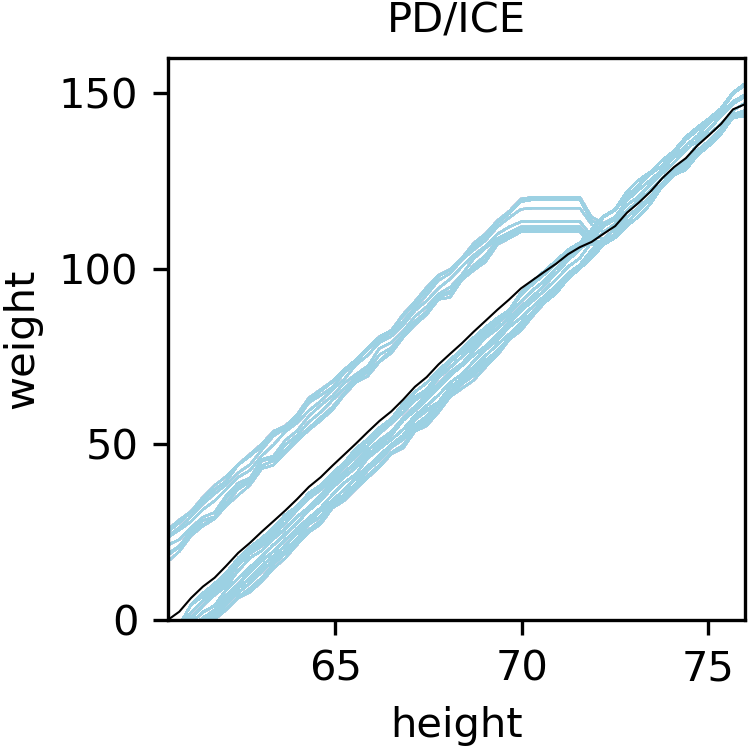
\includegraphics[scale=0.7]{images/height_vs_weight_pdp.png}
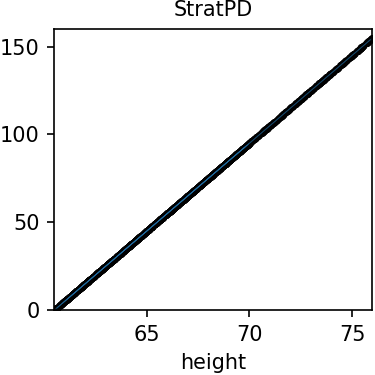
\includegraphics[scale=0.7]{images/height_vs_weight_stratpd.png}
\caption{Plots of height versus weight using synthetic data from Equation \eqref{eq:weight}. The PD/ICE on the left is biased by codependent features since pregnant women, who are typically shorter than men, have a jump in weight.}
\label{fig:height_vs_weight}
\end{center}
\end{figure}

To illustrate how variable codependencies result in misleading PD and ICE plots, consider a body weight data set with observations matching a person's characteristics to a weight in pounds. We discuss the data set details in \secref{sec:codep} (Equation \eqref{eq:weight}), but for the moment, assume that women are slightly shorter on average and are 30 pounds heavier if pregnant. The PD/ICE plot in \figref{fig:height_vs_weight}(a) shows an inaccurate partial dependence where shorter people appear to be slightly heavier per inch of height than those over about 72 inches. At first glance, one may surmise that there is some interesting trend between weight and individuals shorter than 72 inches. The blue ICE lines actually jump up significantly for shorter heights due to the codependence of $x_{height}$, $x_{sex}$, and $x_{pregnant}$. PD and ICE conjure up pregnant males and ask the model to estimate their weight. To be clear, the weight equation has no interaction term with $x_{height}$ and $x_{pregnant}$, but pregnant women, who are typically shorter, have a jump in weight. The \spd{} plot in \figref{fig:height_vs_weight}(b), on the other hand, is not confused by codependence and gives the true partial dependence of weight on height.   The next section describes the \spd{} approach and how it avoids bias from codependent variables.

\section{A stratification approach}

For the remainder of the manuscript, we will use the notation $x_c$ to represent a single variable whose values we observe in column $c$ of $\mathbf{X}$ and we will write $x_{\overline{c}}$ to represent all other variables. A stratification approach to estimate the partial dependence of $y$ on $x_c$ relies on the following two steps. First, the rows of $\mathbf{X}$ are stratified into disjoint collections of observations for which \xnc{} are constant within each collection (ignoring $x_c$). Let $G_j$ be the index set of the $j$th such collection of observations. The resulting pairs $\{(x_{ic},  y_i)\}_{i \in G_j}$ describe how $x_c$ affects $y$, all else being equal. The second step is to fit a local linear regression model of $y$ on $x_c$ over each of the pairs in collection $G_j$: 

% \todo{hmm...what about the dynamic binning we do? we don't fit a single line through each group/leaf of points. see first bullet point of next section 3.1}
%Terence - this is what we are theoretically doing, whereas stratPD is what we do for real data. 

$$y_i = \beta_{0j} + \widehat{\beta}_{G_j} x_{ic} + \epsilon_i, \hskip 1pc i \in G_j.$$

For each collection $G_j$, the estimated coefficient $\widehat{\beta}_{G_j}$ quantifies the partial dependence relationship over the region $[\text{min}(x_{ic}), \text{max}(x_{ic})]_{i \in G_j}$. Ignoring $\beta_{0j}$ (the $y$-intercept) removes the contribution of \xnc{} to $y$ in $G_j$. The regions of $x_c$ space across collections typically overlap.  In order to obtain the overall partial dependence relationship, we can partition $\mathcal{X}$, the domain of $x_c$, into disjoint regions $R_1, \ldots, R_m$. Let $R \in \{R_1, \ldots R_m\}$ be an arbitrary region contained in $\mathcal{X}.$) and let $\mathcal{I} = \{G_j: G_j \bigcap R \neq \emptyset\}$. Then, the partial dependence between $x_c$ and $y$ in a region $R$ is estimated as the weighted average of all coefficients covering that region: 

\begin{equation}\label{eq:truebeta}
	\widehat{\beta}_R = \dfrac{1}{\displaystyle\sum_{G_j \in \mathcal{I}} |G_j|}\displaystyle\sum_{G_j \in \mathcal{I}}|G_j|\widehat{\beta}_{G_j},
\end{equation}

\noindent where $|G|$ is the cardinality of $G$. The collection of regions and coefficients, $\{(R_j, \widehat{\beta}_{R_j}): j = 1, \ldots, m\}$ provide a localized approximation of the partial derivative of the unknown $f(X)$ with respect to $x_c$. If exact stratification is possible, then $\widehat{\beta}_R$ is the minimum variance estimator of the partial dependence of that variable in that region. In this situation, even if the relationship between $y$ and $x_c$ is non-linear, local linear approximation is a well-understood technique for assessing the relationship between variables. 


% Next, talk about how local linear estimation is useful as despite the non-linearity of the relationship of y on X, we can obtain an arbitrarily close approximation using local linear approximation via a Taylor expansion. Namely, (give result). can we then get difference in partial dependence and linear partial dependence in this situation? (ie beta) write this down.}.


Unfortunately, exact stratification is only feasible for two or three variables but breaks down for more variables because it is impractical to find groups of observations that are equal across so many variables.  Nonetheless, stratification is simple, well understood, and clearly isolates the effect of $x_c$ on $y$ from the other features, even in the presence of codependent and interacting features. The only obstacle is a general and practical mechanism for stratifying observations with many variables, which leads us to the primary contribution of this paper.

\subsection{StratPD for numerical variables}\label{sec:numerical}

\spd{} seeks to isolate the local effects of $x_c$ on the observations $\mathbf{y}$ in the presence of confounding variables by estimating its regional effect $\widehat{\beta}_R$ given in (\ref{eq:truebeta}). Due to the challenge of exact stratification in high dimensions, \spd{} instead approximates stratification via a regression tree. The key idea is to relax stratification so that it organizes observations into groups of similar rather than equal observations. To do this, \spd{} trains a decision tree regressor, $T$, as in \cite{CART}, on $(x_{\overline{c}}, {\bf y})$ to stratify observations according to the relationship between \xnc{} and $y$.\footnotetext{The \spd{} algorithm also supports the use of random forests \cite{RF} but primarily to deal with duplicated features, as in \secref{sec:dup}.} Let $L_1, \ldots, L_m$ denote the leaves of the trained tree $T$. Each leaf in the tree represents a region of \xnc{} space and $\{(x_{ic}, y_i)\}_{i \in L_j}$ are the $x_c$ and $y$ observations associated with $L_j$. \spd{} characterizes the relationship between $y$ and $x_c$ on leaf $L_j$ by following two steps:

\begin{itemize}
	\item Partitioning $\{(x_{ic}, y_i)\}_{i \in L_j}$ into disjoint collections (bins of variable width) delimited by the unique $x_c$ values in $L_j$: $B_1, \,\ldots, B_{nbins}$  where $nbins = |\text{unique}(x_c)|-1$. E.g., for unique $x_c$ values $(1,3,4,5)$, the bin regions are $((1,3), (3,4), (4,5))$.
	\item Fitting a simple linear regression of $y$ on $x_c$ from bin $B_k$ to bin $B_{k+1}$ to obtain  $\widehat{\beta}_{B_k}$.
\end{itemize}

Let $\mathcal{J} = \{B_k: B_k \bigcap R \neq \emptyset\}$. We estimate the partial dependence over region $R$ using the weighted average of all $\widehat{\beta}_{B_k}$ that overlap $R$:

\begin{equation}\label{eq:slope}
	{\beta}^{*}_R = \frac{1}{\displaystyle\sum_{B_k \in \mathcal{J}} |B_k|}\displaystyle\sum_{B_k \in \mathcal{J}}|B_i|\widehat{\beta}_{B_k}
\end{equation}

The estimator ${\beta}^{*}_R$ is an estimate of the partial derivative across the region $R$, and so numerically integrating the partial derivatives across $x_c$ space gives a curve representing the contribution of $x_c$ to $y$.  Algorithm 1 encodes the \spd{} process and the full Python 3 source code is available at {\small \url{https://github.com/parrt/stratx}}. 

Revisiting the \spd{} plot in \figref{fig:baths_price}(d), derived from the apartment rent data set, each blue line represents a local slope $\hat{\beta}_B$ through the observations in bin $B$ (which is a partition of $x_c$ space whose \xnc{} features are similar). Lines extend from the minimum to maximum $x_c$ value in a specific $B$.  Because we are interested in the relative contribution of $x_c$ to $y$, \spd{} plots use zero as a $y$-axis baseline. The black dots represent the integration of the partial derivative estimates up to and including each unique $x_c$ value (except the first $x_c$, whose integral value is 0). The partial derivative estimate at an $x_c$ value is the (weighted) average slope of the blue lines emanating from that value. \spd{} does not interpolate between $x_c$ points and so the plot shows dots not lines. 

There are a few situations that deserve special attention. First, as the number of  variables, $p$, increases, stratifying \xnc{} into bins of similar values would normally require more and more data. But decision tree training focuses on those variables that reduce the variance in $y$ (without using $x_c$), leading to leaves that best flatten $y$ subject to hyper parameter ${\it min\_samples\_leaf}$. One can imagine a leaf with some variables in \xnc{} that are not similar, but that would mean that training could not use them to reduce $y$ variance within the leaf. If those variables with unequal values do not explain much $y$ variance, they are unlikely to affect the partial dependence computation for $y$ on $x_c$ in $L$.

Second, if $x_c$ is constant for some leaf $L$, then $L$ does not support any conclusions about how changes in $x_c$ affect $y$ because $x_c$ does not change in $L$.  The observations in $L$, therefore, are {\it non-supporting observations}. Stratification leads to observations that are similar in \xnc{} and, in this case, the observation $x_c$ values are identical. That means that fluctuations in $y$ are likely due to noise or exogenous variables not included in the data set. Such a leaf does not contribute bin coefficients, $\hat{\beta}_B$, in Algorithm 1 to the overall slope for the leaf's $x_c$ region. This situation occurs most often when $x_c$ contains integers.

Third, it's reasonable to ask why we use unique $x_c$ values within each $L$ as the bin edges, rather than splitting $x_c$ into fixed-width bins.  This was our original approach because of its simplicity, but it required another hyper parameter, such as $nbins$, and led to high proportions of non-supporting observations in some data sets. When all or most of the $x_c$ values are discrete integers, some choices of $nbins$ would lead to virtually all bins in all leaves having a single $x_c$ value. \spd{} would generate a questionable plot due to lack of available $\hat{\beta}_B$. Also, binning integers leads to awkward bins, such as 1.8 to 3.2 bedrooms or dayofweek 1.3 to 2.1.  Using the unique $x_c$ values themselves avoids a second hyper parameter and guarantees that bins do not have non-supporting observations unless the entire leaf has a single unique $x_c$.

Partial dependence through stratification also works for data sets with categorical variables in \xnc{}, given a suitable similarity measure between observations that supports categorical variables, but identifying an appropriate categorical similarity measure is a well-known issue.  Decision trees, however, support categorical variables easily and effectively by treating categories as unique integers. Observations with categorical variables that end up in the same leaf are likely to be similar (\cite{RFunsup}). Algorithm 1, therefore, works without modification for \xnc{} containing categorical variables encoded as unique integers. When the column of interest, $x_c$, is categorical, however, a new algorithm is required. For this situation, we introduce the \cspd{} method, which is described and evaluated in \appdxref{appendix:catstrat}.

\subsection{Partitioning feature space with trees and forests}\label{sec:partitioning}

Stratification of $(x_{\overline{c}}, y)$  into regions of similar observations is at the core of our approach so it's worth examining how \spd{} partitions feature space in more detail.  The goal is to find groups of extremely similar \xnc{} values in $({\bf X}, {\bf y})$ so fluctuations in $y$ are due solely to changes in $x_c$. Such groups yield pieces of the partial dependence of $y$ on $x_c$. \spd{} looks for similar observations because, beyond a few variables, it's not possible to stratify observations by equal \xnc{} values. 

Inventing a new partitioning strategy is unnecessary because decision trees already exist that can tesselate \xnc{} feature space into small hypervolumes of similar observations. If a hypervolume is tight enough, then \xnc{} values are very similar and the slope of regression lines through unique $x_c$ values of $(x_{L}, y_L)$ is a good estimate of the partial derivative of $\frac{\partial y}{\partial x_{c}}$ across leaf L.  If the \xnc{} volume for leaf $L$ is too large, then \xnc{} observations in $L$ are not similar enough to conclude that changes in $y$ are due to $x_c$ alone. By default, our Python implementation of \spd{} creates decision trees with at least 10 observations per leaf, but depending on $y$, post-training leaf size is unbounded. The $x_c$ space within each leaf is then split into bins, dictated by the unique $x_c$ values, in preparation for piecewise linear approximation.

Decision trees are known to overfit, which was the impetus for the invention of Random Forests(tm) (RF) \cite{RF}.  The use of decision trees by default rather than RFs in \spd, therefore, might seem an odd choice. Using RFs was our initial approach and the \spd{} algorithm and source code still support RFs. (The only change required to support RFs is to iterate over all leaves from all trees, rather than the leaves of a single tree, to collect local $x_c$ slopes.)  Decision trees are sufficient for partial dependence, however, because the goal is to understand the population described by the training set, not to make predictions; that is what models are for. The one exception is that multiple trees are needed to handle features in \xnc{} that are identical or highly-correlated with $x_c$ (see \secref{sec:dup}).

To reduce overfitting, RFs bootstrap and select split variables from a subset of all variables in order to create uncorrelated trees. But, that means increasing bias of individual trees to some degree because each tree is trained on roughly 2/3 of the training data and without considering some of the variables. Because our goal is to group together {\em all} observations that are similar in {\em all} \xnc{} variables, it is counterproductive to bootstrap and select variables from a subset. Because partial dependence is meant to explore existing $(\bf X, y)$ data rather than make predictions on future data, there's no point in sacrificing accuracy for generality. 

For the data sets we examined during the preparation of this paper, moving from a decision tree to a random forest with various numbers of trees did not affect the partial dependence results; \figref{fig:weight_ntrees} and \figref{fig:rent_ntrees} show some typical results. The integrated partial derivative curves identified by the black dots do not change as the number of trees increases from left to right.  In one simulation run for the rent data set, we did see a difference in the partial dependence dots for an extreme value of $x_{bedrooms}$ with very few $y$ values, but it's unclear which plot is correct for this real data set. (The answer is unclear because the true partial dependence for a variable of an unknown function is unknown.)

The blue lines representing piecewise partial derivative estimates increase in number as the number of partitions (leaves) increases.  Note that the variance of the partial derivative estimates is wider for RFs than for a single decision tree. This is expected because the decision tree leaves contain all observations in a feature space hypervolume and so the estimate will be less biased; RF leaves have at most 2/3 of the observations for the same hypervolume, the bootstrapping population size estimate. The education versus weight plots in \figref{fig:weight_ntrees} illustrate this most clearly. The blue ``cone'' around the partial dependence dots widens as the number of trees increases.  

Increasing the number of trees does not improve accuracy and increases the time complexity linearly in the number of trees, which is roughly what we see in practice.  For example, using a single decision tree to partition a 10,000-observation rent data set sample and generate a plot takes .3s on our 4.0Ghz processor but about 8s for 30 trees (first row, far right of \figref{fig:rent_ntrees}).

\begin{figure}[htbp]
\begin{center}
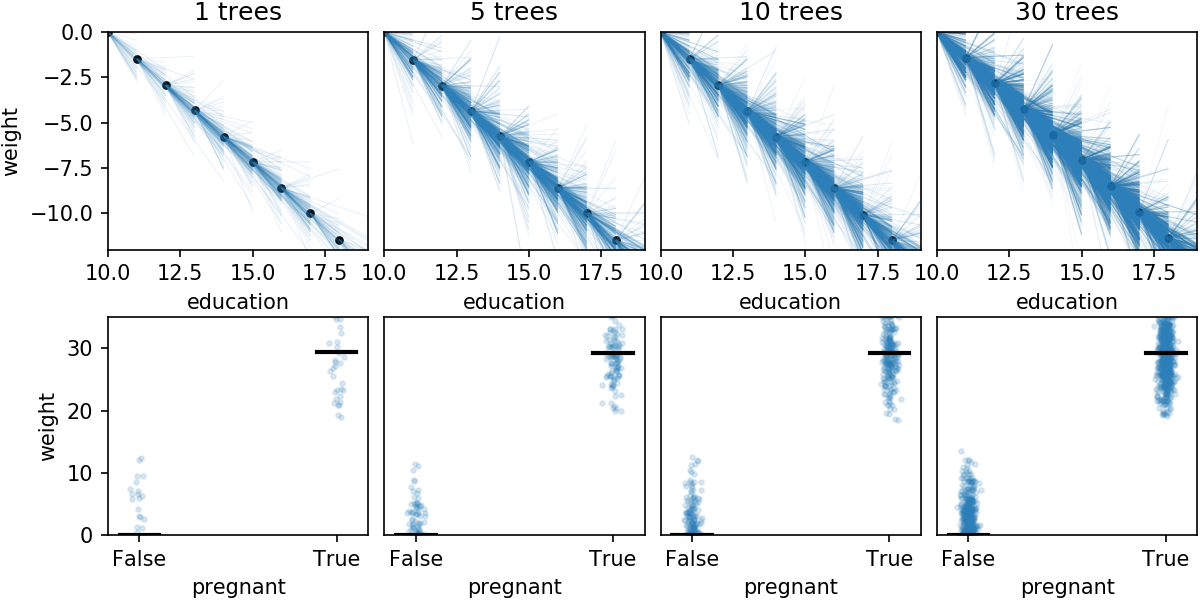
\includegraphics[scale=0.55]{images/education_pregnant_vs_weight_ntrees.png}
\caption{A comparison of single decision tree versus bootstrapped random forests with 5, 10, and 30 trees using synthetic data (2000 observations) from Equation \eqref{eq:weight}. The top row shows no advantage to using more trees numerical $x_c$ variables and the bottom row shows the same is true for categorical $x_c$. ${\it min\_samples\_leaf}$ is 5 for education and 10 for pregnant.}
\label{fig:weight_ntrees}
\end{center}
\end{figure}

\begin{figure}[htbp]
\begin{center}
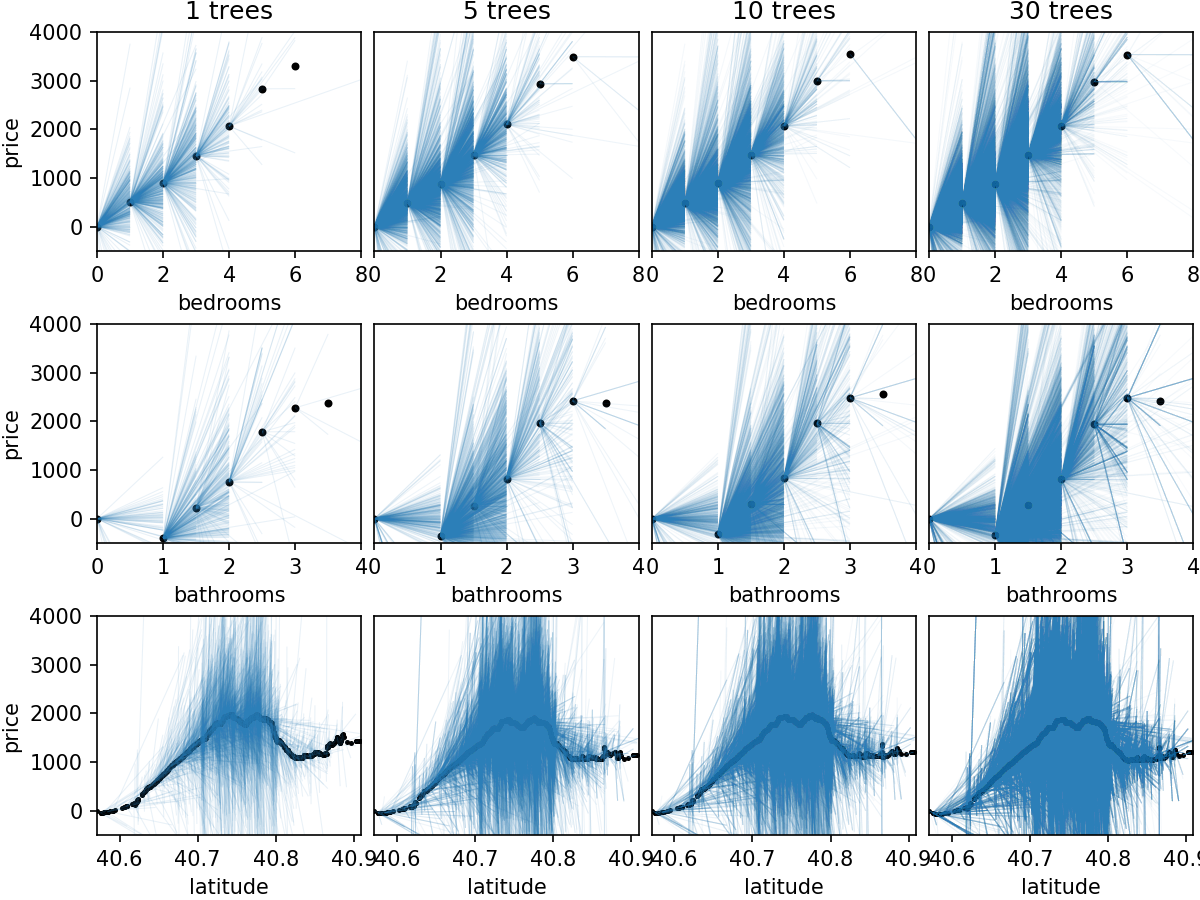
\includegraphics[scale=0.55]{images/rent_ntrees.png}
\caption{A comparison of single decision tree versus bootstrapped random forests with 5, 10, and 30 trees using NYC apartment rent data set. The three rows illustrate variables bedrooms, bathrooms, and latitude versus price. These graphs suggest there is no advantage to using random forests over decision trees.}
\label{fig:rent_ntrees}
\end{center}
\end{figure}

Decision trees choose feature space hypervolumes that minimize the variance in $y$, but $y$ is technically not needed to partition \xnc{} into similar regions. \cite{RFunsup} described how to use random forests in an unsupervised fashion by considering the original $\bf X$ matrix as class 1 and a synthesized $\bf X'$ as class 2, which works equally well for individual decision trees, at least for this stratification application. $\bf X'$ is just $\bf X$ with each $x'_j$ column bootstrapped (drawn randomly with replacement) from $x_j$ in $\bf X$, effectively sampling from $x_j$'s marginal distribution. \figref{fig:rent_weight_unsup} shows typical results from three variables from the rent data set and two variables from the synthesized weight data set.  The left column shows unsupervised partitioning of $\bf X$ and the right column shows the usual supervised partitioning with $(\bf X, y)$. The results are very similar but the variance of the partial derivative estimates for the unsupervised case appears to be a bit wider. The \cspd{} unsupervised and supervised plots for categorical variable $x_{\it pregnant}$ in \figref{fig:rent_weight_unsup}(b) are virtually indistinguishable. 

\figref{fig:boston_unsup} illustrates a case where unsupervised partitioning is less stable and less accurate: $x_{\it AGE}$ versus $x_{\it MEDV}$ (median house value) from the well-known Boston housing data set. The figure shows a marginal plot then the unsupervised and supervised \spd{} plots (and finally the PD/ICE plot). To increase stability for the unsupervised version, we used 20 trees with bootstrapping. But, in the end, there's no reason to perform unsupervised partitioning when $y$ is always available. (Partial dependence makes no sense without $y$.) 

The point is that partitioning \xnc{}  with a decision tree is more about $\bf X$ than $\bf y$, which strengthens our claim of model-independence. \spd{} does not rely on a user's model, never makes predictions from internal models, and can even get away with partitioning feature space without $\bf y$.

\begin{figure}[htbp]
\begin{center}
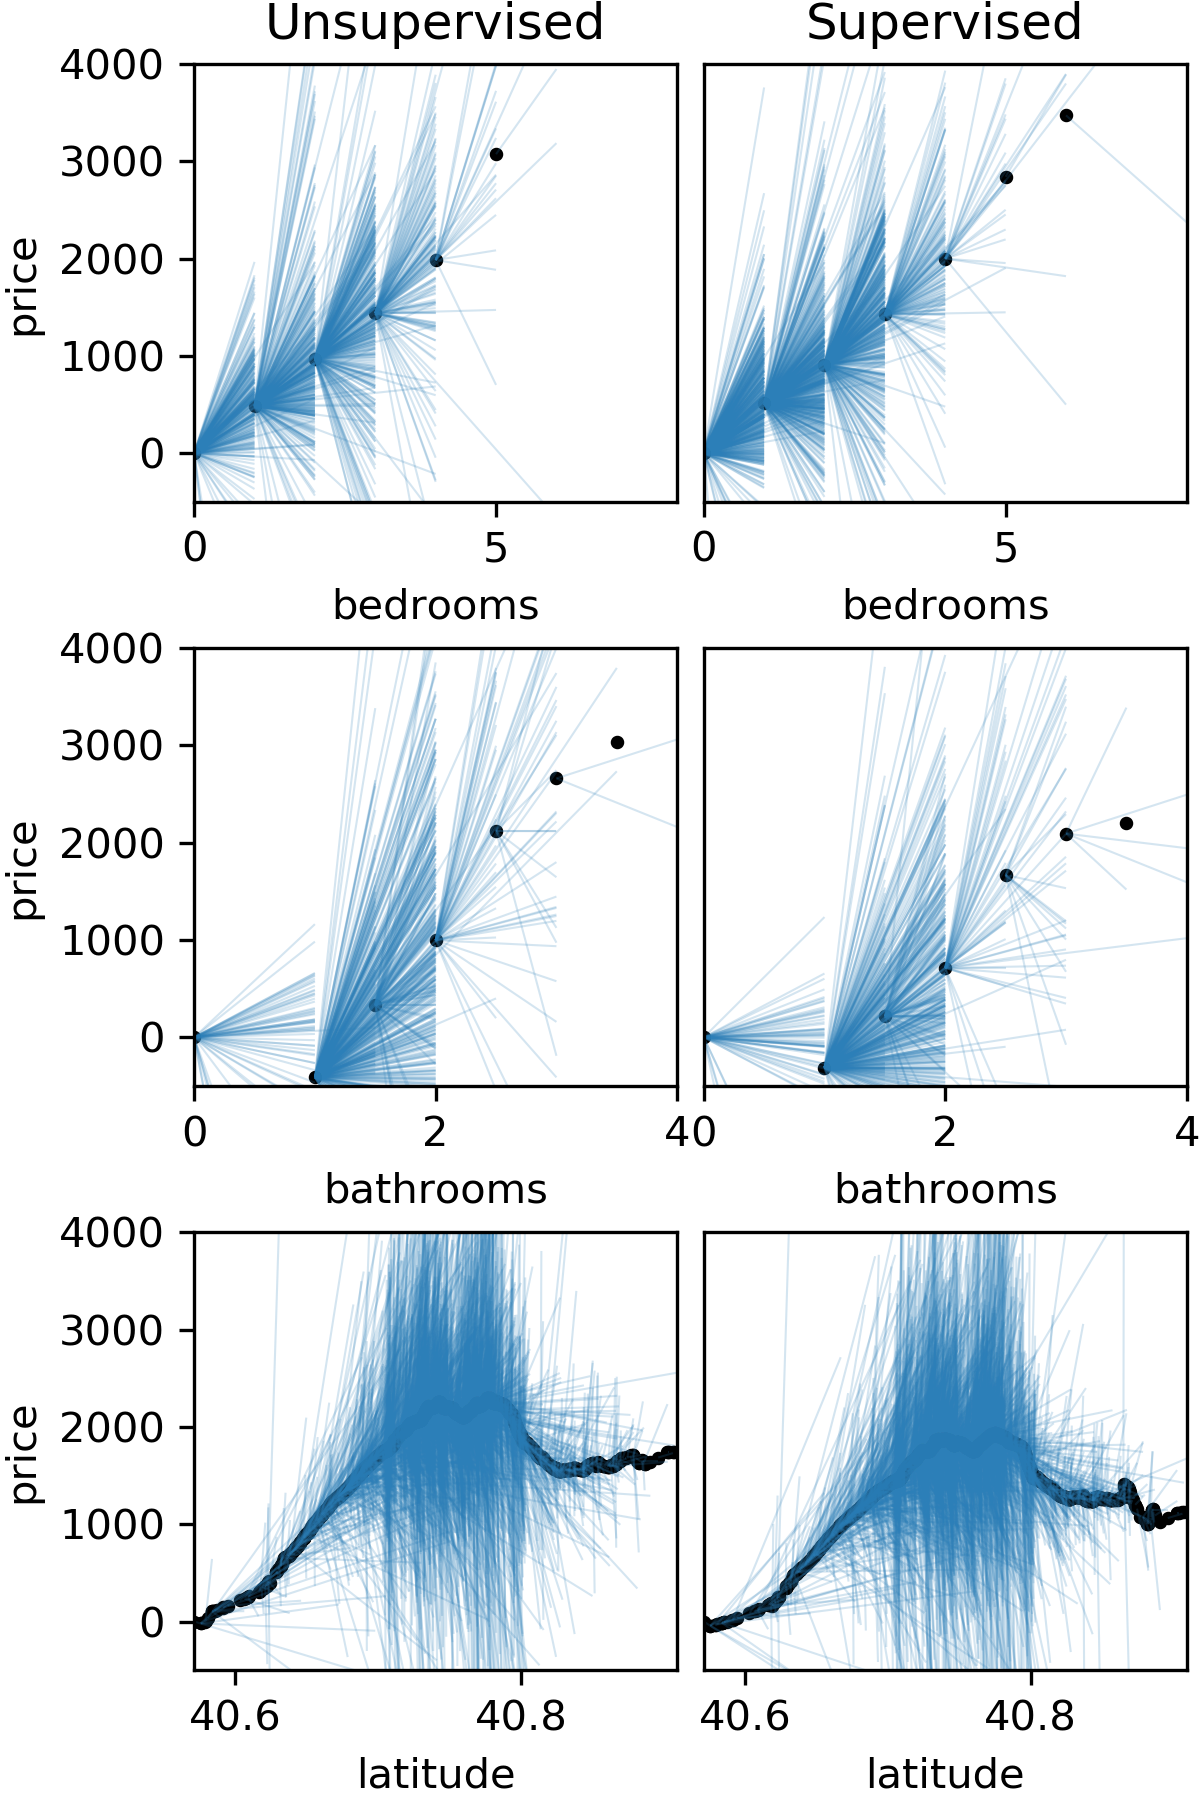
\includegraphics[scale=0.7]{images/rent_unsup.png}
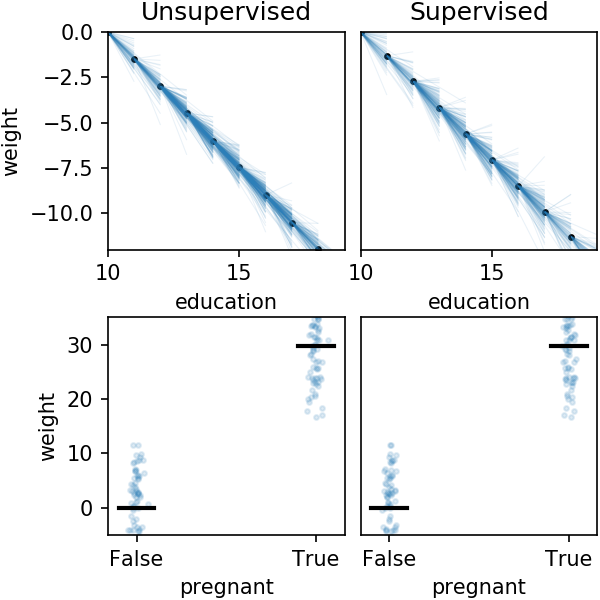
\includegraphics[scale=0.7]{images/weight_unsup.png}
\caption{Comparing the effect of partitioning \xnc{} space with (supervised) and without (unsupervised) $\bf y$ data using apartment rent data and synthetic body weight data. These graphs suggest that \xnc{} can often be successfully partitioned without $\bf y$.}
\label{fig:rent_weight_unsup}
\end{center}
\end{figure}

\begin{figure}[htbp]
\begin{center}
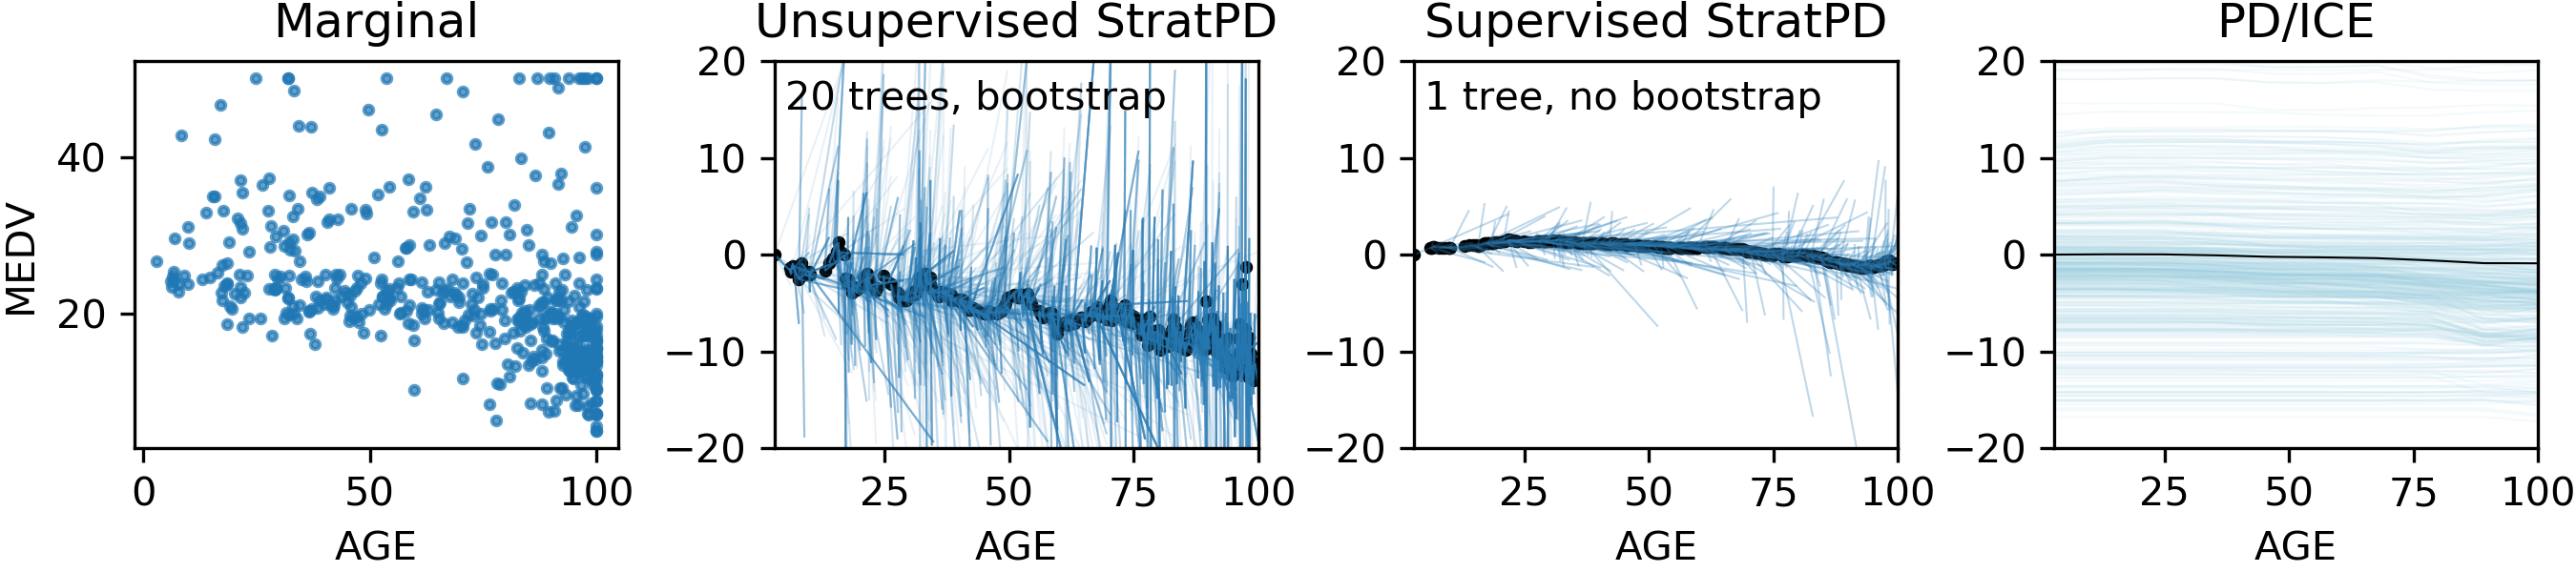
\includegraphics[scale=0.7]{images/boston_unsup.png}
\caption{A demonstration that unsupervised partitioning (without $\bf y$ data) leads to unstable partial dependence graphs. Using a random forest instead of a single decision tree improved results, but the supervised \spd{} is still better.}
\label{fig:boston_unsup}
\end{center}
\end{figure}


 
\section{Experimental Results}\label{sec:applications}

This paper proposes a stratification approach to isolating the effect of $x_c$ on target $y$ and has shown a few \spd{} and \cspd{} plots to highlight their advantages over PD and ICE plots. In this section, we provide more examples on synthetic and real data sets, investigate the effect of noisy data, and examine how \spd{} deals with edge cases arising from unusual \xnc{} partitioning.  All plots in this paper, including the PD/ICE plots, were generated using the Python {\tt stratx} library and script {\tt genfigs.py} (in the github repository). (PD/ICE plots were derived from RF models with 100 trees and {\it min\_samples\_leaf}=1). 

We begin by reproducing graphs from \cite{ICE}, starting with their equation in which independent variables $x_2$ and $x_3$ interact:

\begin{equation}\label{eq:bigX}
y = 0.2x_1 - 5x_2 + 10x_2\mathbf{1}_{x_3 \geq 0} + \epsilon~~~~~x_1, x_2, x_3 \sim U(-1,1), \epsilon \sim N(0,1)
\end{equation}

\noindent \figref{fig:bigx_stratpd} shows the \spd{} plots in the left column for $x_2$ and $x_3$ and the PD/ICE plots in the right column. As \cite{ICE} points out, the PD plot (top row, right side) shows no effect of $x_2$ on $y$ predictions, but the ICE plot makes it clear that the apparent lack of PD effect is due to an interaction or interactions with other variables that cancel out. In this case, we know from Equation \eqref{eq:bigX} that $x_3$ ``turns off'' $10 x_2$ roughly half the time ($x_3 \sim U(-1,1)$), yielding an $x_2$ contribution to $y$ of $5 x_2$ not $-5 x_2$. The \spd{} plot also shows a relatively flat partial dependence line, although it is much smoother than the PD/ICE line. The noise, $\epsilon \sim N(0,1)$, is about as large as the ``data'' and so there is nontrivial variation from simulation to simulation; curves should be taken as clues not absolute truth. Because \spd{} draws the approximate partial derivatives of $y$ along $x_2$, there is a roughly regular pattern of alternating lines of roughly slope 4 or 5, which is what we would expect since $\frac{\partial y}{\partial x_2}$ is either 5 or -5.

\begin{minipage}[t]{0.45\textwidth}
\vspace{1em}
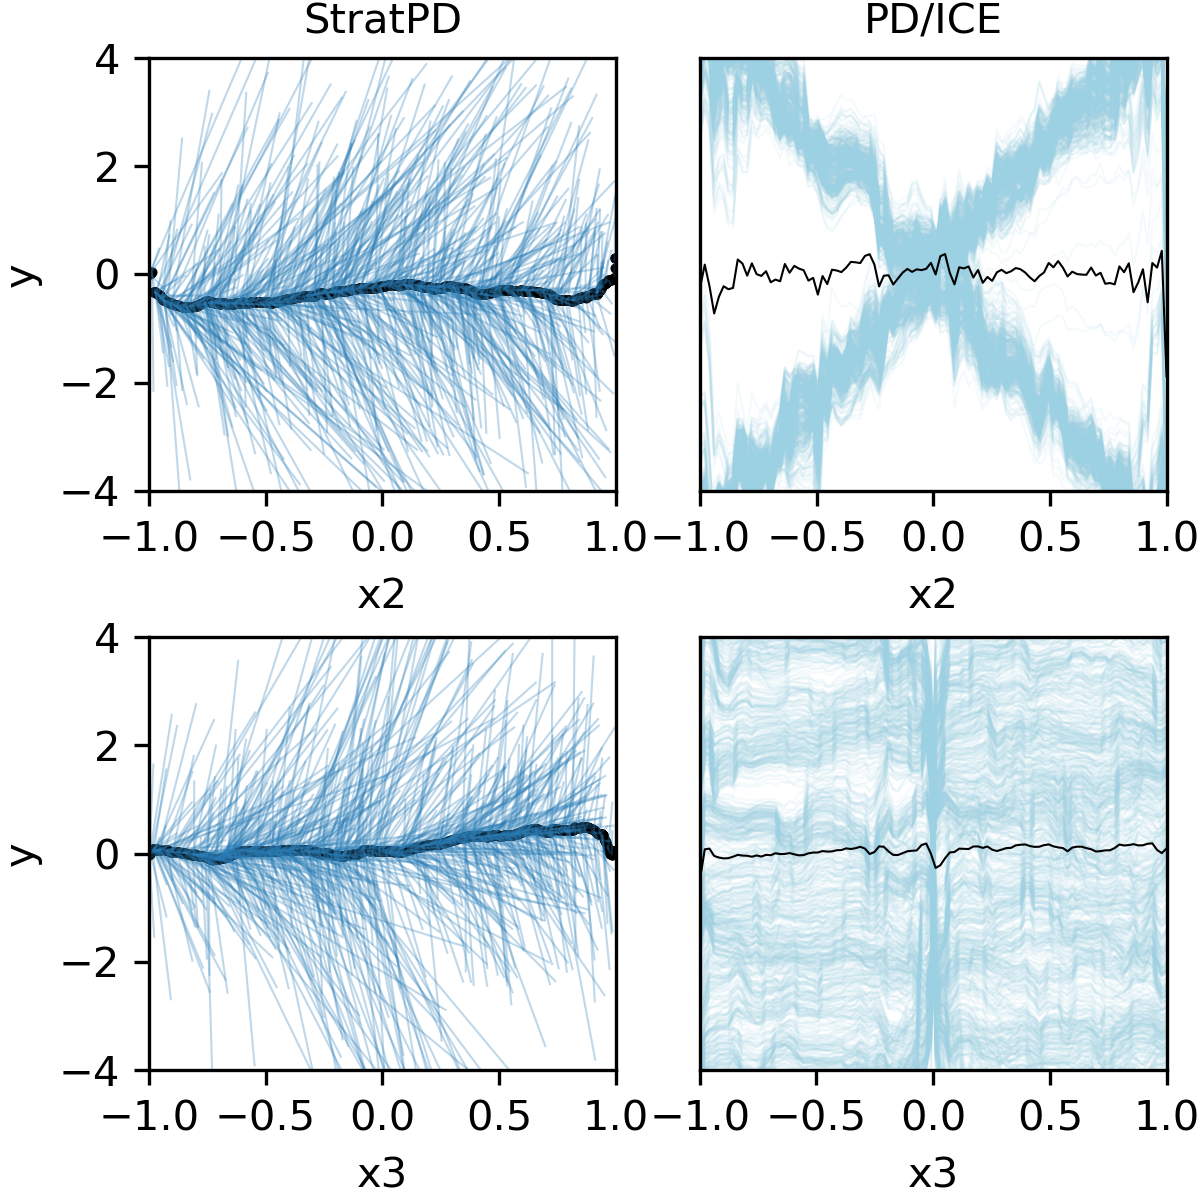
\includegraphics[scale=0.7]{images/bigx.png}
\captionof{figure}{Plots of $x_c=x_2$ and $x_c=x_3$ from 1000 observations generated from Equation \eqref{eq:bigX}. \spd{} plots in the left column and PD/ICE in the right column. Both algorithms show a roughly flat partial dependence curve. PD/ICE shows a clear interaction pattern for $x_2$, as does \spd{} but \spd{}'s interaction pattern is less obvious. \vspace{1em}}
\label{fig:bigx_stratpd}
\end{minipage}
\hfill
\begin{minipage}[t]{0.45\textwidth}
\vspace{1em}
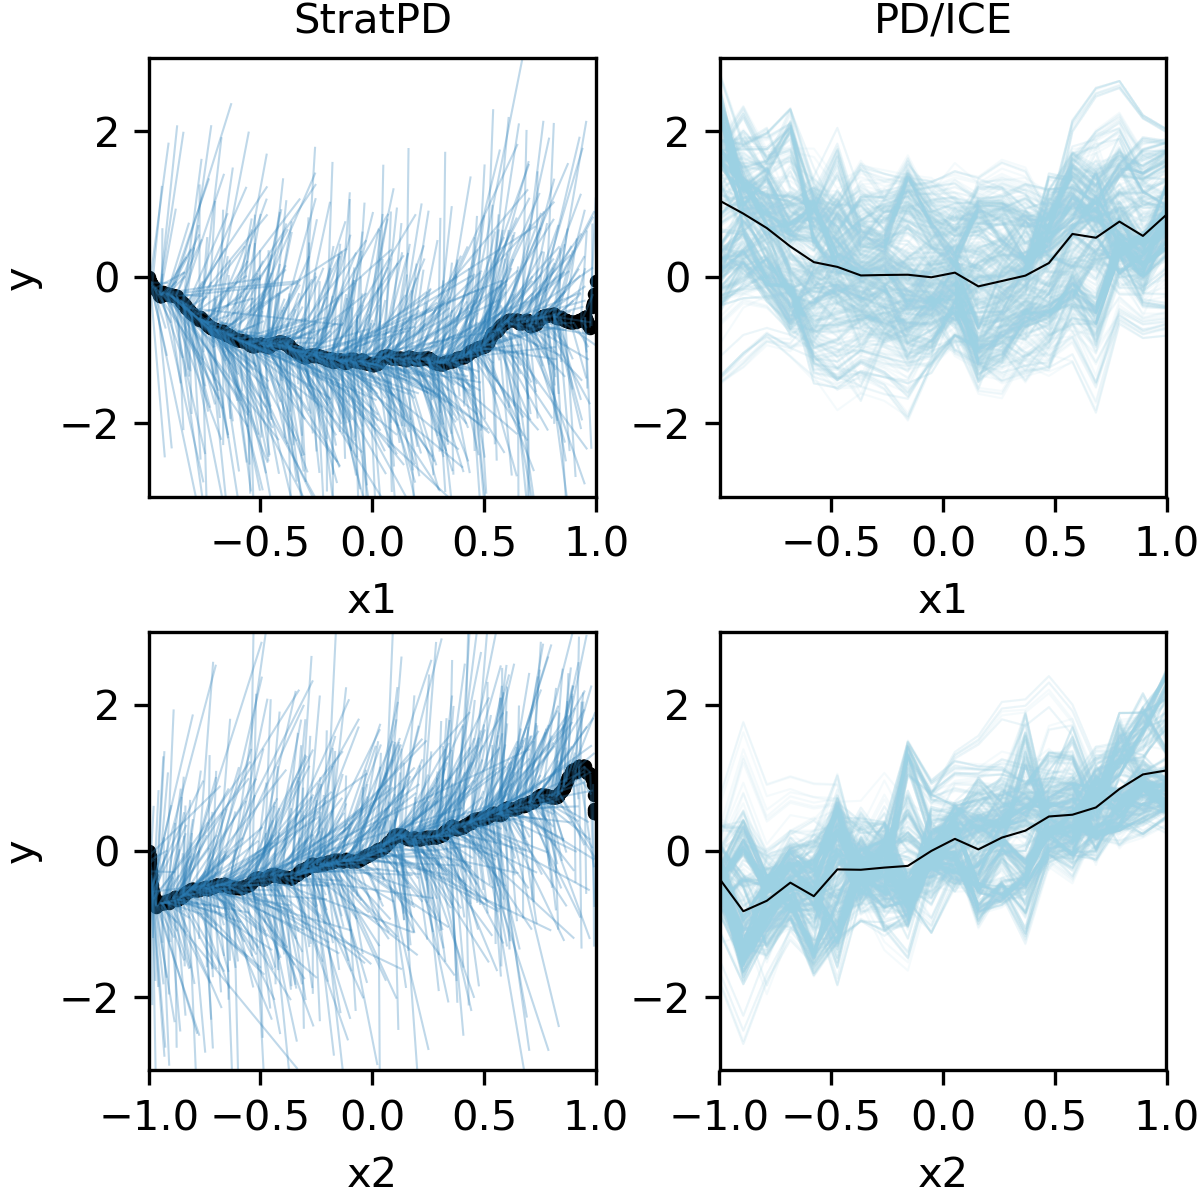
\includegraphics[scale=0.7]{images/additivity.png}
\captionof{figure}{Plots of $x_c=x_1$ and $x_c=x_2$ from 1000 observations generated from Equation \eqref{eq:parabola}. \spd{} plots in the left column and PD/ICE in the right column. Both algorithms show the appropriate parabolic and linear partial dependence curves. {\it min\_samples\_leaf}=10 for both to smooth over noise.}
\label{fig:additivity_stratpd}
\end{minipage}

The partial dependence curves in the \spd{} and PD/ICE plots for $x_3$ in \figref{fig:bigx_stratpd} are also relatively flat lines because $\frac{\partial y}{\partial x_3}=0$ when $x_3 < 0$ and $10 x_2$ when $x_3 \ge 0$. Since $x_2 \sim U(-1,1)$, $10 x_2$ contributes positive and negative noise to $y$, which the \spd{} plot exhibits with partial derivative lines at random angles (much more random than for the \spd{} plot of $x_2$ versus $y$).

\cite{ICE} also demonstrate the use of ICE plots for additivity assessment using a second-order equation:

\begin{equation}\label{eq:parabola}
y = x_1^2 + x_2 + \epsilon~~~~~x_1, x_2 \sim U(-1,1), \epsilon \sim N(0,1)
\end{equation}

\noindent We will use this equation to demonstrate that the local, nonparametric method of \spd{} can identify quadratic relationships, as shown in the left column of \figref{fig:additivity_stratpd}; the right column shows the equivalent PD/ICE plots. The \spd{} plots for $x_1$ and $x_2$ are smoother, which can make the partial dependence relationships more pronounced visually than in the PD/ICE plots.  The effect of $x_2$ on $y$ should be a line with slope 1, as shown in the second row of \figref{fig:additivity_stratpd}. Both PD/ICE and \spd{} plots give reasonable depictions of the linear relationship. To smooth out the noise, we set \spd{} hyper parameter ${\it min\_samples\_leaf}$ to 50, which means stratification partitions \xnc{} space into leaves with at least 50 observations; the default is 10. We examine noise more closely in \secref{sec:noise}.

\subsection{Isolating the effect of codependent features on $y$}\label{sec:codep}

None of the variables used in Equations \eqref{eq:bigX} and \eqref{eq:parabola} are codependent and ICE plots have no problem exposing interactions and generating accurate PD curves.  PD/ICE make the assumption that variables are independent, however, and the plots become less accurate as codependence grows.  To compare \spd{} to PD/ICE for codependent variables, we synthesized a body weight data set with 2000 observations drawn from the following equation with codependence between features.

\begin{equation}\label{eq:weight}
\begin{array}{rll}
y & = &120 + 10(x_{height} - min(x_{height})) + 30x_{pregnant} - 1.5x_{education}\\
\vspace{-10pt}\\
\multicolumn{2}{r}{\text{where}} & x_{sex} \sim Bernoulli(\{M,F\}, p=0.5)\\
                    & & x_{pregnant} = \begin{cases}
                                               Bernoulli(\{0,1\},p=0.5) & \text{ if } x_{sex} = F\\
                                               0 & \text{ if } x_{sex}=M\\
                                               \end{cases}\\
                    & & x_{height} = \begin{cases}
                                               5*12+5+ \epsilon & \text{ if } x_{sex}=F,~ \epsilon \sim U(-4.5,5)\\	
                                               5*12+8 + \epsilon & \text{ if } x_{sex}=M,~ \epsilon \sim U(-7,8)\\
                                               \end{cases}\\
                    & & x_{education} = \begin{cases}
                                               12 + \epsilon & \text{ if } x_{sex}=F,~ \epsilon \sim U(0,8)\\	
                                               10 + \epsilon & \text{ if } x_{sex}=M,~ \epsilon \sim U(0,8)\\
                                               \end{cases}
\end{array}
\end{equation}

Because of the codependence between $x_{pregnant}$ and $x_{height}$ via $x_{sex}$, \figref{fig:height_vs_weight} demonstrated that the PD/ICE plot incorrectly shows shorter people as heavier on average. PD/ICE conjures up unlikely observation such as pregnant males, resulting in biased ICE lines.

As another example of isolating codependent variable effects, compare the \spd{} and PD/ICE plots in \figref{fig:education_vs_weight} showing number of years of education versus weight. Weight is related to education by slope -1.5, so a perfect partial dependence graph would show a drop of 12 pounds over 8 years of education. The PD/ICE plot captures only about two thirds of that relationship, whereas, the \spd{} plot gets the true education-weight relationship.  Female observations have at least 12 years of education, versus 10 for males, so $x_{education}$ and $x_{sex}$ are codependent, though, there is no interaction term. The fact that women are shorter on average biases the education-weight PD/ICE plot because the baseline weight is lower from which the education contribution is  subtracted.

\begin{figure}[htbp]
\begin{center}
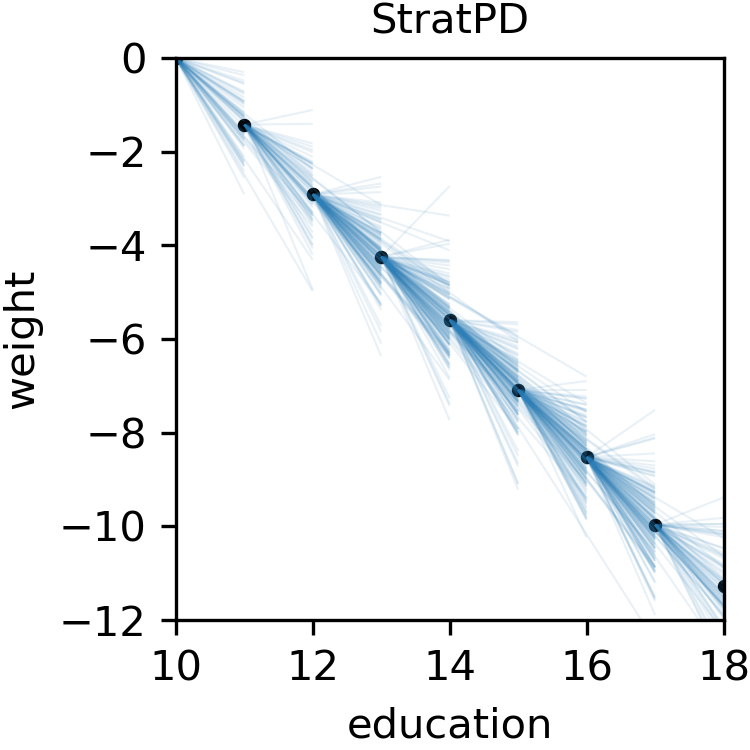
\includegraphics[scale=0.7]{images/education_vs_weight_stratpd.png}
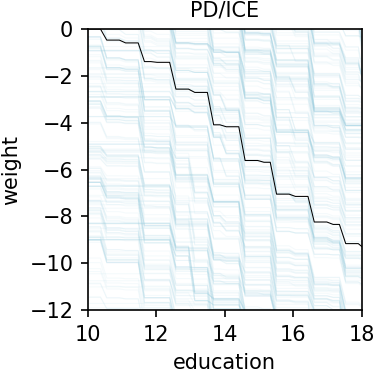
\includegraphics[scale=0.7]{images/education_vs_weight_pdp.png}
\caption{Plots of education versus body weight using 2000 observations from Equation \eqref{eq:weight}. The \spd{} clearly identifies the linear relationship and with the proper slope of -1.5, whereas the PD/ICE plot has a more shallow slope.}
\label{fig:education_vs_weight}
\end{center}
\end{figure}

Because the ``signal-to-noise ratio'' is low in the bodyweight data set, we set hyper parameter ${\it min\_samples\_leaf}=2$ to partition \xnc{} into very tight regions, leaving at least two observations from which estimate the change in $y$ over $x_c$ space. Tight regions increase the likelihood that $y$ fluctuations in each leaf are due solely to changes in $x_c$.

\subsection{The effect of model choice on PD/ICE plots}

Perhaps the biggest issue with PD and ICE plots is that they rely on predictions from a user-provided model $\hat{f}(\bf X)$, and different models make different assumptions and have different strengths and weaknesses.  Users must choose the appropriate model for the data set and properly tune the models, otherwise ICE trendlines are untrustworthy. \figref{fig:4var} shows marginal plots, \spd{} plots, and PD/ICE plots for a 4-variable normal distribution with center $(6, 6, 6, 6)$ and covariance matrix:

\[
\left(
\begin{array}{cccc}
1 & 5 &.7 & 3\\
5 &1 &2 &.5\\
.7 &2 & 1 & 1.5\\
3 &.5 &1.5 &1\\
\end{array}
\right)
\]

\noindent where $y$ is related to the variables by:

\begin{equation}\label{eq:4var}
y = x_1 + x_2 + x_3 + x_4
\end{equation}

\noindent The last four rows show PD/ICE plots from four different models: random forests (100 trees), support vector machines ($\gamma=1/4$), ordinary least squares linear models, and $k$-nearest neighbor ($k=5$).  Because this data set is essentially skewed noise, we increased the number of data points per leaf during stratification of \xnc{}: ${\it min\_samples\_leaf} = 20$.

\begin{figure}[htbp]
\begin{center}
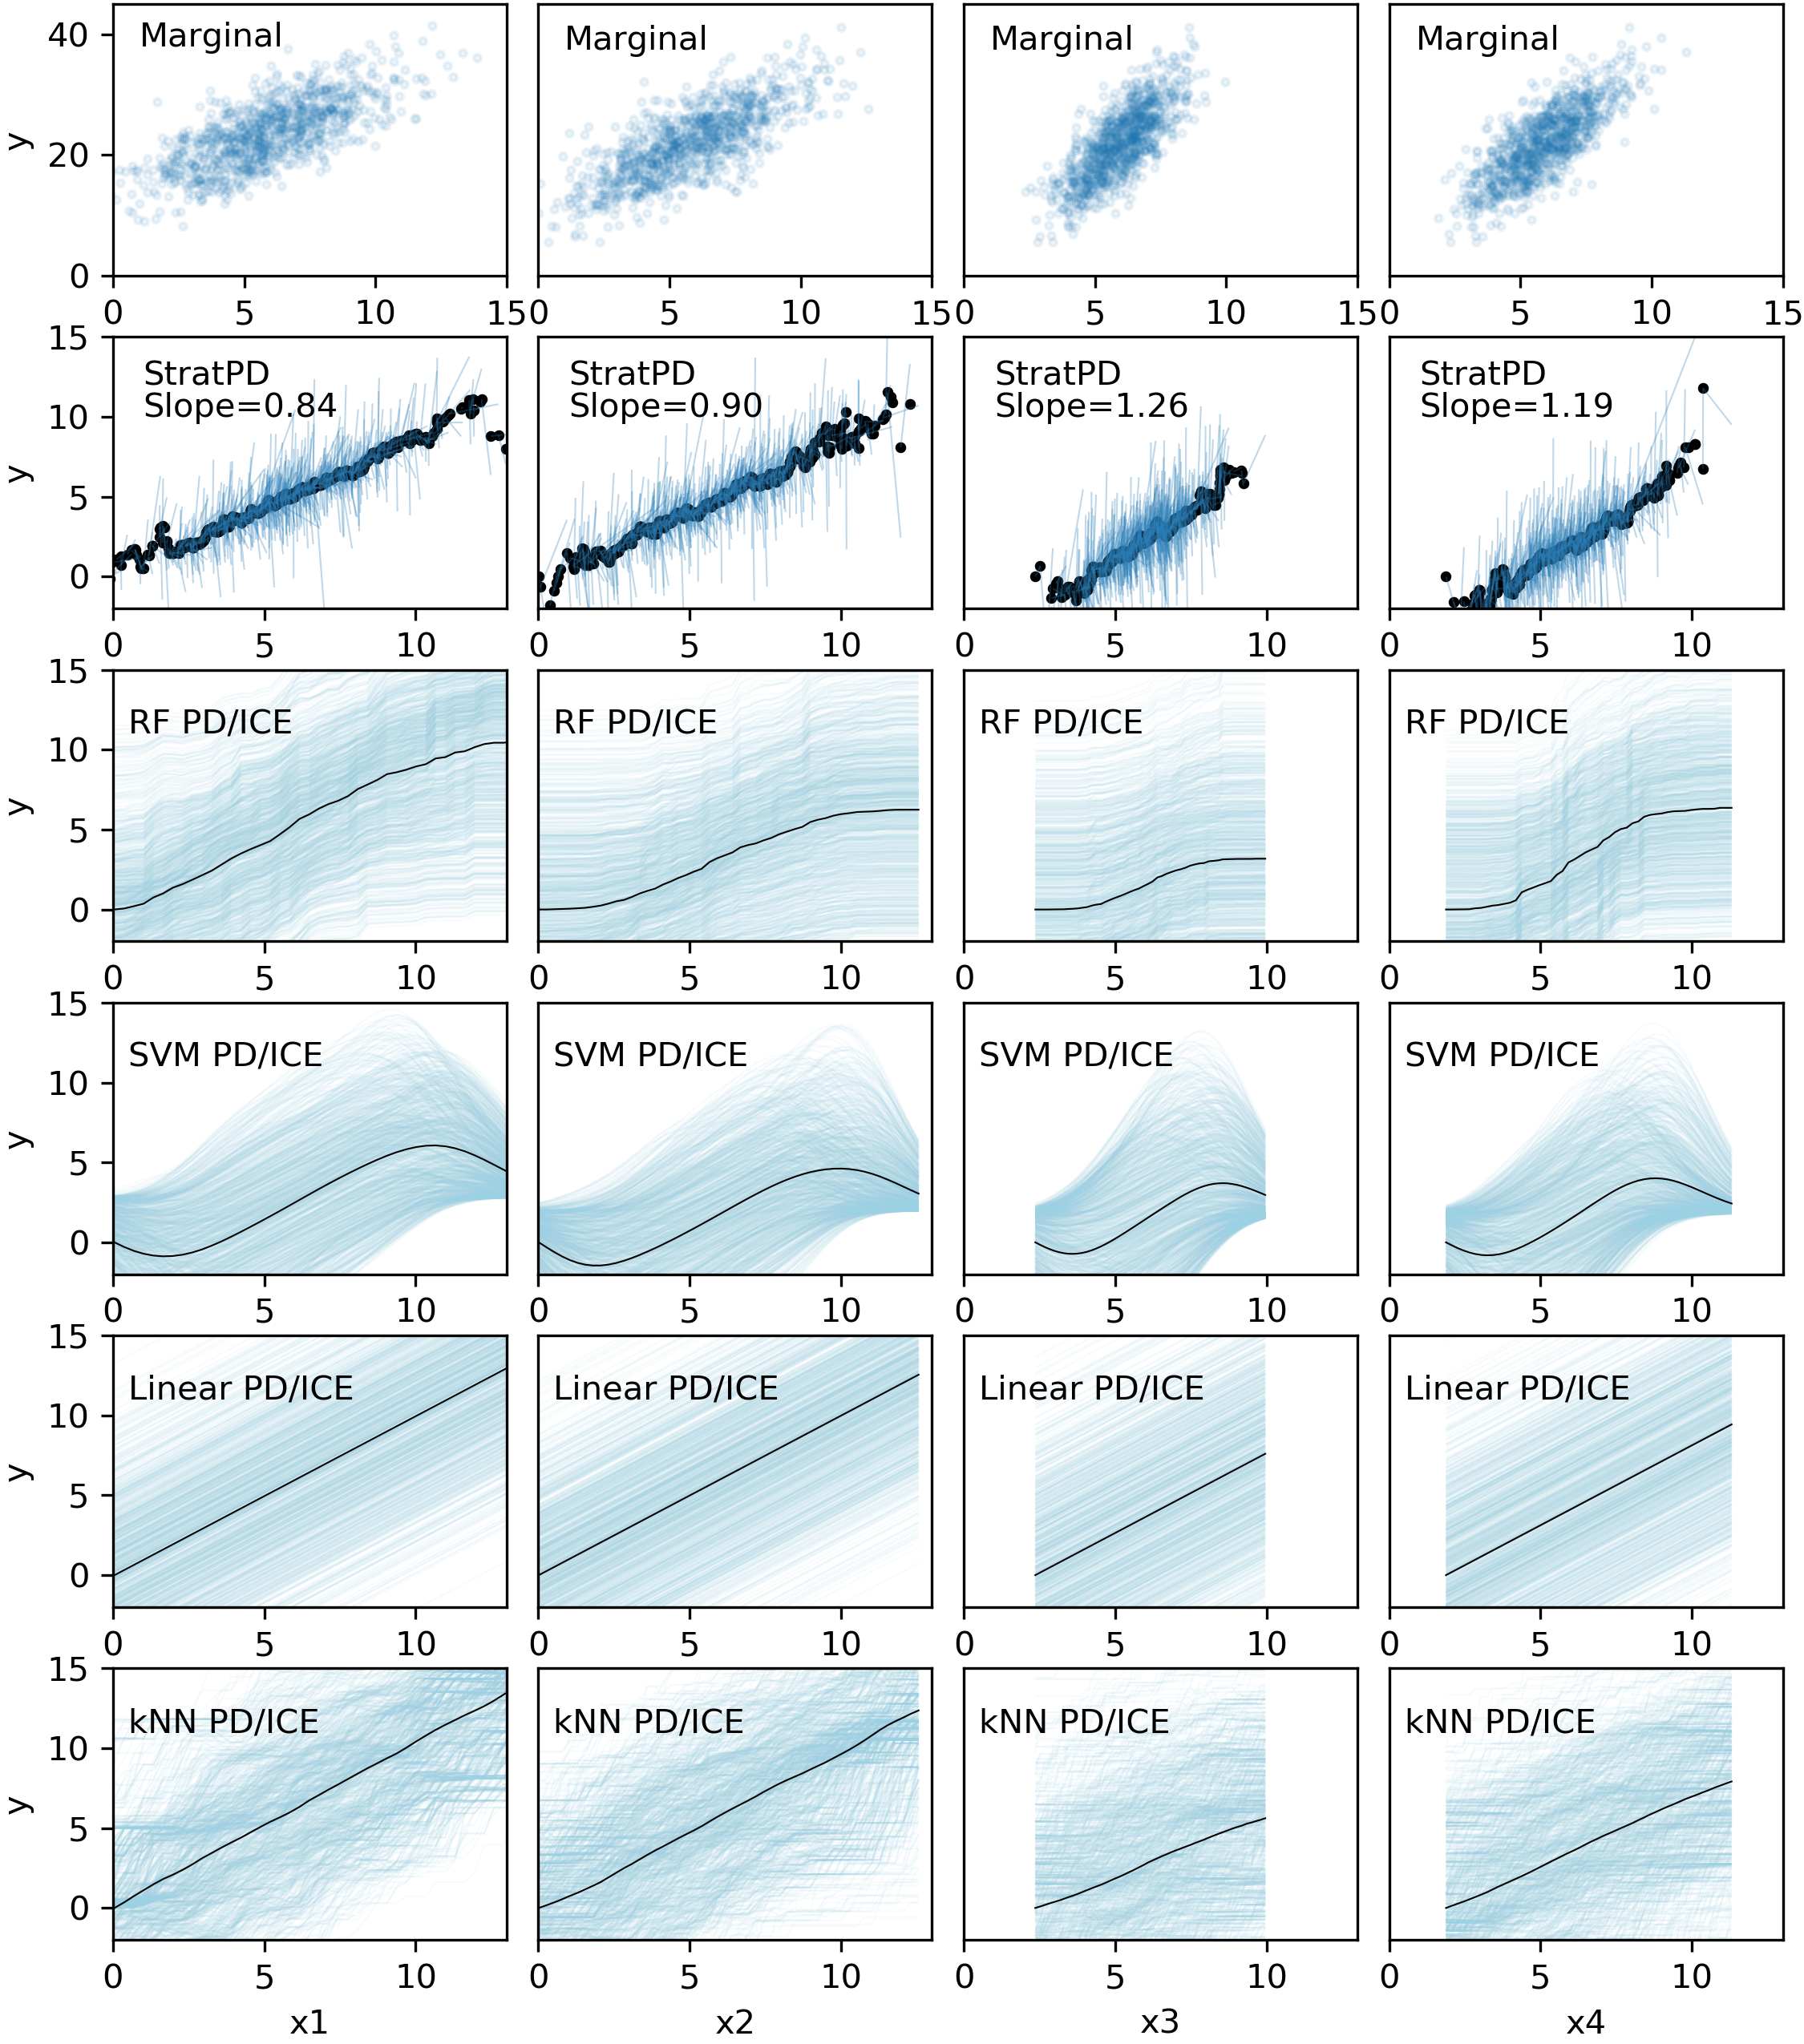
\includegraphics[scale=0.6]{images/multivar_multimodel_normal.png}
\caption{Marginal, \spd{}, and PD/ICE plots using 1000 operations from Equation \eqref{eq:4var} and a variety of fitted models for PD/ICE. The plots clearly demonstrate that PD/ICE results are highly dependent upon the model chosen by the user. \spd{} gets the appropriate linear partial dependence with nearly the correct slope of 1.0 for each variable.}
\label{fig:4var}
\end{center}
\end{figure}

Because $\frac{\partial y}{\partial x_{c}} = 1$ for all $x_c$, the partial dependence curves should be lines with slope 1.  The second row of \figref{fig:4var} has \spd{} plots that show linear relationships and the slopes are close to 1.  The PD/ICE plots derived from RF and SVM models show distinct flattening or curving behavior at the edges because the variables are codependent. Models are presented with highly unlikely combinations of $x_i$ variables that are outside of the training data and are forced to extrapolate outside of their support range.  The linear model does very well because it assumes the relationship is linear and, therefore, extrapolates linearly without issue. The nearest neighbor model also captures the linear relationship well but underestimates the partial dependence slope for $x_3$ and $x_4$.
 
\subsection{Duplicated columns require multiple decision trees}\label{sec:dup}

Isolating $x_c$ from codependent variables in \xnc{} through decision tree stratification works well in our experiments unless $x_c$ is a linear function of a variable in \xnc{}. In that case, stratification hammers out variation in $x_c$, as if the decision tree were trained on $(\bf X, y)$ not (\xnc, $\bf y$). To simulate this pathological situation, we duplicated $x_{\it bathrooms}$ from the rent data set and generated the \spd{} and PD/ICE plots in \figref{fig:baths_dup}. The first column shows \spd{} and PD/ICE plots without a duplicated column and the second column shows the result of duplicating $x_{\it bathrooms}$. Both plots show much reduced partial dependence of $y$ on the highly-predictive variable $x_{\it bathrooms}$. In the case of \spd{}, the stratification process groups the data by apartments with similar bathrooms and so it shows less partial dependence for the duplicated bathrooms variable.   There are many fewer lines in the \spd{} plot for the duplicated column because half of the data does not support any conclusions about partial dependence: most of the leaves contain a unique $x_c$ value.

\begin{figure}[htbp]
\begin{center}
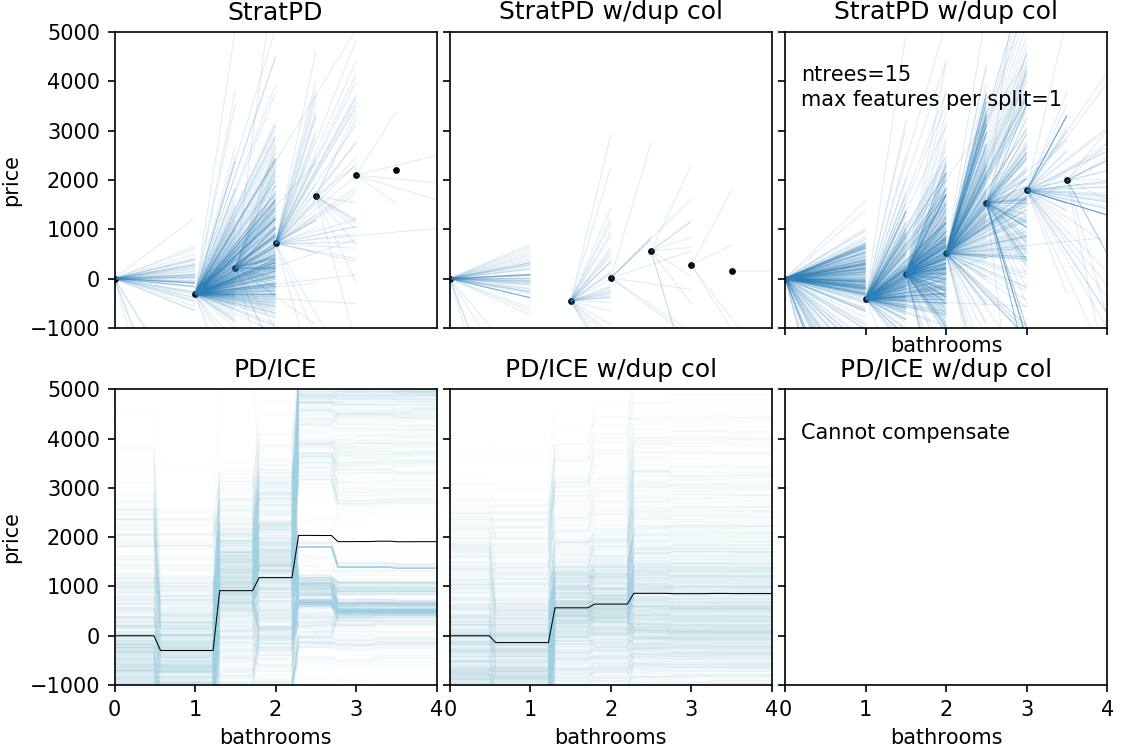
\includegraphics[scale=0.6]{images/bathrooms_vs_price_dup.png}
\caption{The effect of duplicating the predictive $x_c$ explanatory variable using 10,000 observations of \textasciitilde49k from the rent data set. The first column shows \spd{} and PD/ICE plots without the duplicated variable and the second column shows plots after duplicating the $x_c$ variable. To partially compensate, users can increase the number of trees but without bootstrapping and setting hyper parameter {\it max\_split\_features} to 1, as shown in the third column. PD/ICE has no way to compensate for the duplicated $x_c$ variable.}
\label{fig:baths_dup}
\end{center}
\end{figure}

The problem with the PD/ICE plot is not because of codependence between $x_{\it bathrooms}$ and its duplicate. Instead, the PD/ICE is lower because of the nature of this data set and the way RFs train. With two identical variables, decision nodes that split on one of those variables will choose between them with 50\% probability.  To create ICE trendlines, only one of the duplicate variables changes through $x_{\it bathrooms}$ space, which means that roughly half the tree decision nodes will lead to predictions that ignore the shifted $x_c$ variable.  This has the effect that the model underestimates rent prices.  For example, given an observation with $x_{\it bathrooms}=1$, (simplifying slightly) half the trees in the forest would predict rent appropriate for one bathroom even when the trend line shifts the $x_c$ bathrooms to 4. It would be possible to switch models in an effort to overcome this issue, but many models do not support duplicated or highly-correlated variables.

To compensate for duplicate columns, \spd{} supports the use of RFs rather than a single decision tree to stratify \xnc{} space. \spd{} uses decision trees by default rather than conventional RFs because bootstrapping is not important and, in fact, increases bias as the individual trees are working on 2/3 of the data set. The third column, top row in \figref{fig:baths_dup} shows the \spd{} plot resulting from the use of 15 trees ($ntrees=15$) and limiting decision node variable choice to one of two randomly-selected variables at each split (${\it max\_split\_features}=1$).  Restricting the number of variables available during node splitting prevents partitioning from relying too heavily on the duplicate of $x_c$, leading to a number of leaves that vary in $x_c$ from which \spd{} can estimate the partial dependence.

\subsection{Compensating for noise}\label{sec:noise}

To explore the effect of irrelevant variables on \spd{} plots, we introduced a noise column ($x_{\it noise} \sim U(0,50)$) to the rent data set. Because decision trees ignore variables with low predictive power, stratification automatically ignores irrelevant or noise columns.  \figref{fig:beds_noise} shows \spd{} and PD/ICE plots for the original data set and the data set with a noise column. Both approaches are unaffected by the introduction of the noise column, but that is true for PD/ICE because this particular plot was also derived from a random forest. PD/ICE plots derived from models that are confused by noise columns would not be accurate.

\begin{figure}[htbp]
\begin{center}
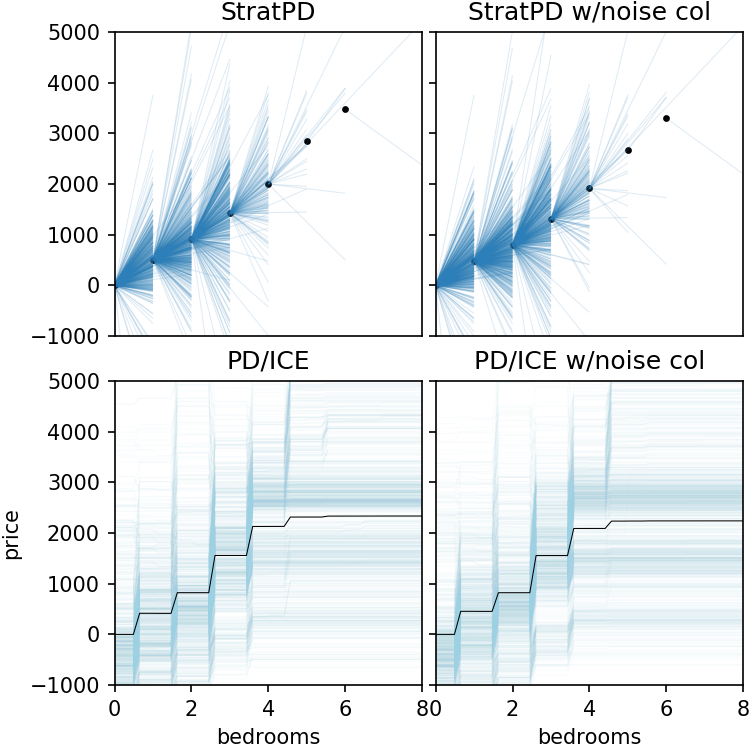
\includegraphics[scale=0.6]{images/bedrooms_vs_price_noise.png}
\caption{The effect of adding a variable of noise to $\bf X$ using 10,000 observations of \textasciitilde49k from the rent data set. The first column shows \spd{} and PD/ICE plots without the noise variable and the second column shows plots after introducing the noise variable. The \spd{} plot ignores the noise variable as does PD/ICE because that plot was derived from a random forest model that deals well with irrelevant variables.}
\label{fig:beds_noise}
\end{center}
\end{figure}

\begin{figure}[htbp]
\begin{center}
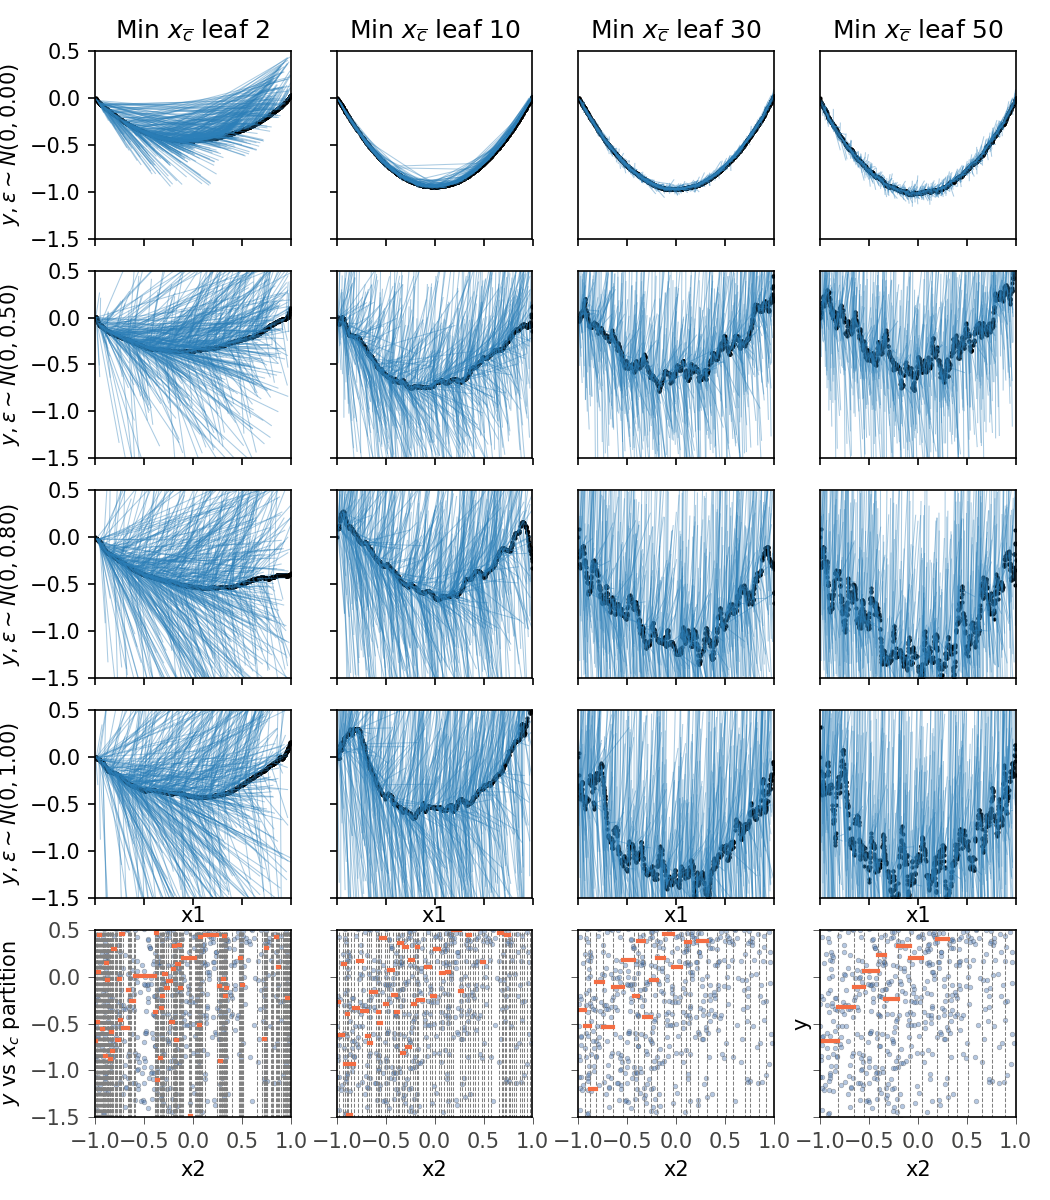
\includegraphics[scale=0.7]{images/meta_additivity_noise.png}
\caption{The effect of increasing amounts of Gaussian noise on \spd{} plots using 1000 observations from Equation \eqref{eq:parabola}. As the signal-to-noise ratio drops, \spd{} is less able to pick out the parabola.}
\label{fig:meta_noise}
\end{center}
\end{figure}

Overcoming noisy predictive columns or noisy $y$ sometimes requires tuning hyper parameter ${\it min\_samples\_leaf}$. \figref{fig:meta_noise} shows the effect of changing ${\it min\_samples\_leaf}$ on \spd{} plots at different noise levels for the Equation \eqref{eq:parabola} quadratic data set.   The bottom row shows decision tree partitioning of \xnc{}=$x_2$ space.  The first row represents the baseline where $y$ omits Gaussian noise. \spd{} easily picks out the quadratic relationship of depth 1 in [-1,1] and is insensitive to increases in the partitioning leaf size for \xnc{}=$x_2$.  As more and more Gaussian noise is added to $y$, the \spd{} plots become more erratic, particularly for larger partitioning leaf size as that increases the likelihood that \xnc{} is influencing $y$. Note that the amplitude of the noise, standard deviation 1.0, in the second to last row is equal to the effect size of a parabola with depth 1.0.  Partially from graphs like this, we chose the default ${\it min\_samples\_leaf}$ hyper parameter  to be 10.

\subsection{\spd{} and \cspd{} applied to real data} 

We have shown \spd{} operating on a real New York City apartment rent data set in figures such as \figref{fig:baths_price} and \figref{fig:rent_ntrees}.  This section shows both \spd{} and \cspd{} plots for another real Kaggle data set, \cite{bulldozer}, concerning auction sales of used bulldozers.  Of the 52 features, we selected three codependent features: YearMade, MachineHours, and ModelID. \figref{fig:bulldozer} shows marginal plots for the three variables versus bulldozer sale price in the first column, the \spd{} and \cspd{} plots in the second column, and PD/ICE in the third column. The nominal variable ModelID axis in the third row was sorted by sale price. To reduce overplotting and to reduce ICE plotting time, we use the most recent 10,000 records after dropping those with missing values or zero machine hours. Random forests for PD/ICE were trained with 20 not 100 trees. The  PD/ICE plot for ModelID shows just 1000 of the roughly 1500 unique values (and still takes 5 minutes to generate).

\begin{figure}[htbp]
\begin{center}
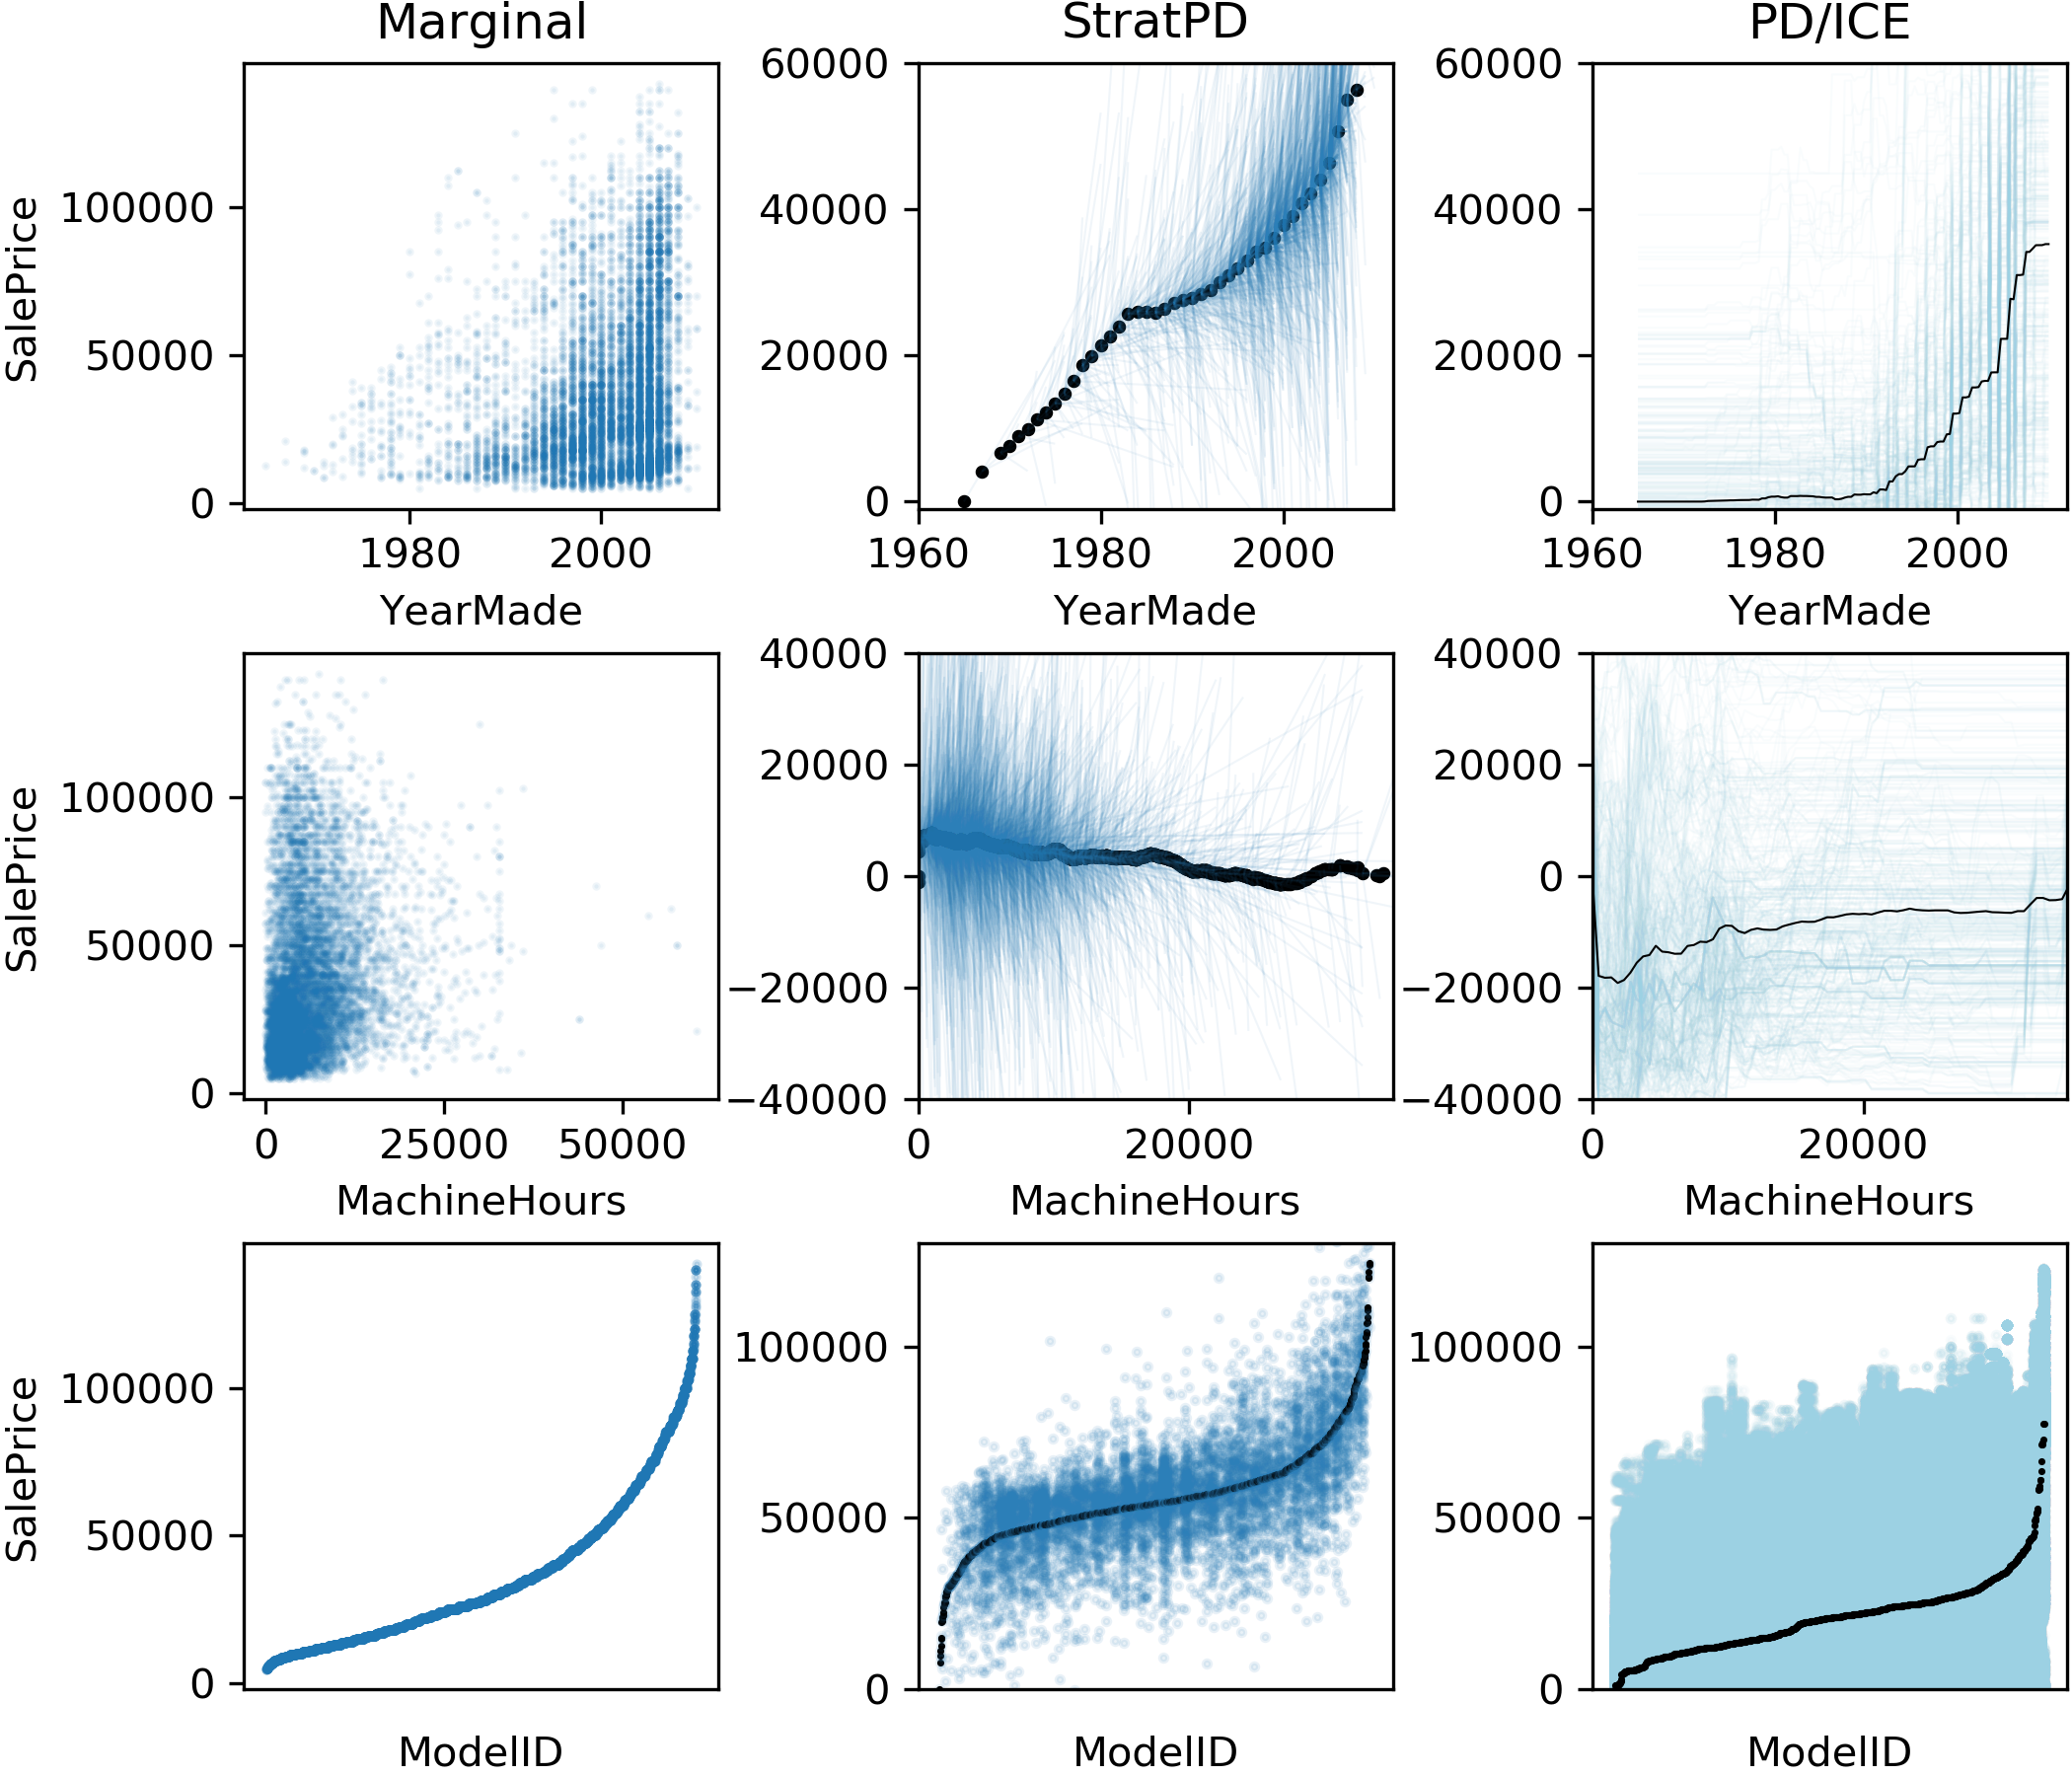
\includegraphics[scale=0.7]{images/bulldozer.png}
\caption{\spd{} and PD/ICE plots for 10,000 of \textasciitilde400k observations from the bulldozer data set. The first row shows YearMade versus price, the second shows MachineHours versus price, and the third shows ModelID versus price. The \spd{} plots are plausible, certainly more plausible than the PD/ICE plots; e.g., it is unlikely that bulldozer sale prices rise as wear-and-tear (MachineHours) increases. The random forest used by PD/ICE had an out-of-bag $R^2$ of about 0.77 using just those three features.}
\label{fig:bulldozer}
\end{center}
\end{figure}

As this is a real not synthesized data set, the true partial dependence curves are unknown. Further, using only three features means the stratification approach will not be able to cancel out contributions to the sale price from the unused features. (Nontrivial feature engineering would be required to extract predictive features from the other variables and these three get an ``out of bag'' metric of $R^2=0.77$) Such exogenous variables could be influencing the \spd{} and \cspd{} plots to be more similar to the marginal plots than is correct.

Both the \spd{} and PD/ICE plots show a price decay as bulldozers age, though the \spd{} plot is more linear for bulldozers older than about 1980 and the PD/ICE plot looks more exponential. It is possible that the linear decay shown in the \spd{} plot is more accurate because it differs significantly from the PD/ICE plot, which will suffer from the codependence of these three features. For example, the ICE lines shift the MachineHours feature into impossible observations, such as bulldozers that have been in use before they were manufactured or bulldozers sold before their ModelID existed. It is clear from both plots that there is a great deal of price variability as bulldozers age, given the \spd{} slope lines and ICE lines.  The \spd{} plot (but not the PD/ICE plot) illustrates that there were many fewer bulldozers for sale that were manufactured before 1990 given the scarcity of lines in that range (which it is consistent with the marginal plot).

The \spd{} plot for MachineHours is linear with a slight negative slope in the $x_c$ region where there is sufficient data, which is plausible.  The slope lines indicate a high degree of variability that often cancel out, very much like the ``big X'' pattern in \figref{fig:additivity_stratpd}. The PD/ICE plot shows a gradual increase in price as bulldozers get more use, which is highly unlikely, and also shows an immediate drop of about \$30,000 for machines that get used for a few hours. Given that the average bulldozer price is about \$36,000, that initial drop is likely due to variable codependence rather than bulldozers truly losing (then regaining) most of their value immediately.

The \cspd{} plot for ModelID (sorted by sale price) closely matches the marginal plot, which could be the true relationship or due to variables omitted from \xnc{} or even omitted from $\bf X$. The PD/ICE plot also shows that some models are much more expensive than others, but is much more curvilinear.

\subsection{Pathological partitioning issues}\label{sec:tuning}

There is a pathological case to consider during \xnc{} partitioning when training yields a decision tree with very large leaves, perhaps hundreds or thousands of observations.  This can happen when \xnc{} contains a single categorical variable or when the only strongly-predictive variable in \xnc{} is categorical.  The weather data set from Equation \ref{eq:weather} is a case in point. (See the marginal plot in \figref{fig:dayofyear_vs_temp}(a).) Choosing $x_c$=$x_{dayofyear}$, means \xnc{}=\{$x_{state}$,$x_{year}$\} and categorical $x_{state}$ accounts for the largest changes in temperature.   A decision tree splitting on just $x_{\it state}$, for example, would group all 365 daily temperature observations for a single state into just one leaf. (The marginal plot shows the complete sine waves but from the side, edge on.)   The \spd{} plot in \figref{fig:dayofyear_vs_temp}(b) clearly shows the sinusoidal temperature fluctuations over the year while holding the state and year constant. The PD/ICE plot also identifies the noisy sine waves, as shown in \figref{fig:dayofyear_vs_temp}(c).

\begin{figure}[htbp]
\begin{center}
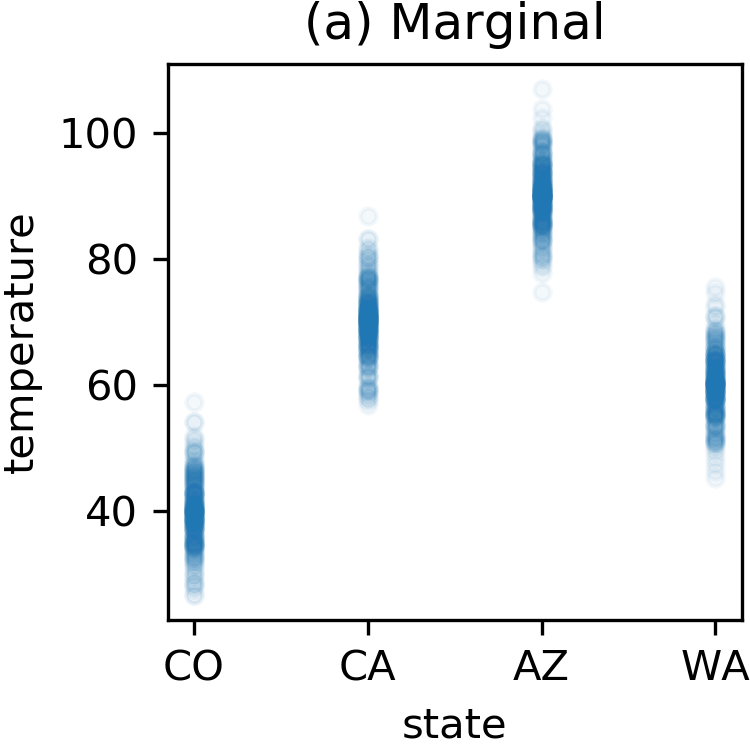
\includegraphics[scale=0.7]{images/state_vs_temp.png}
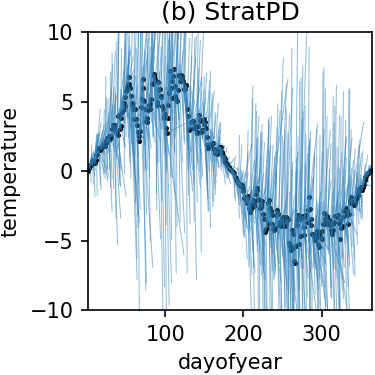
\includegraphics[scale=0.7]{images/dayofyear_vs_temp_stratpd.png}
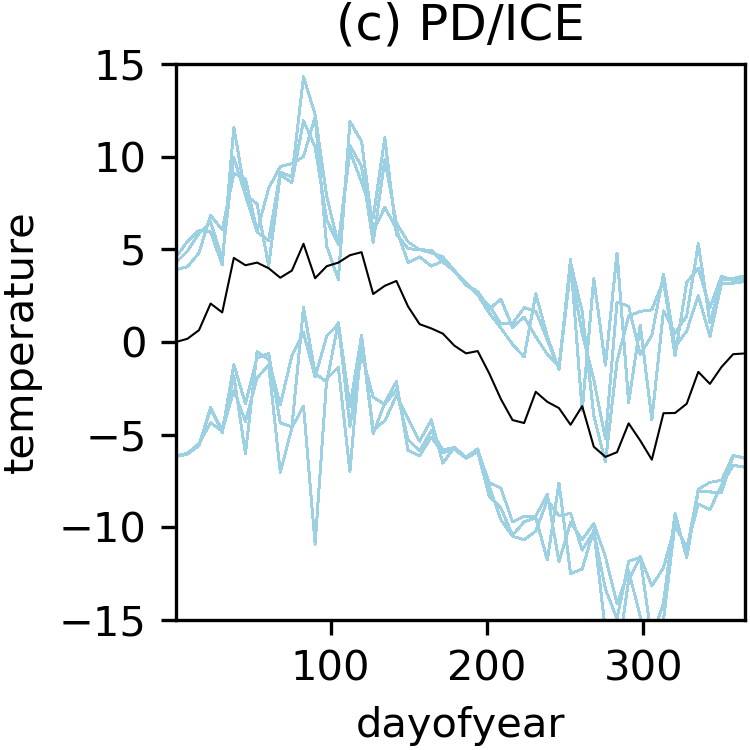
\includegraphics[scale=0.7]{images/dayofyear_vs_temp_pdp.png}
\caption{Pathological partitioning of \xnc{} space can leave extremely large leaves. For $x_c$ of dayofyear, \spd{} partitions the state variable, leaving leaves with at least a year of temperature data. \spd{} and PD/ICE plots both identify the sinusoidal relationship from three years of data using Equation \eqref{eq:weather}.}
\label{fig:dayofyear_vs_temp}
\end{center}
\end{figure}

\subsection{Hyper parameter tuning}

The key idea behind \spd{} is stratification and so hyper parameter {\it min\_samples\_leaf} is  important to the operation of the algorithm; the default is 10. Larger values lead to more observations in each $x_c$ bin, which gets more accurate $\hat{\beta}_B$ estimates. As {\it min\_samples\_leaf} gets larger, however, it is more likely that variables from \xnc{} are contributing to $y$.  Smaller values lead to much more confidence that fluctuations in $y$ are due solely to $x_c$, but smaller bins lead to higher variance among the $\hat{\beta}$ estimates. Fewer observations per leaf can also cause stratification to miss nonlinear and complex behavior between $y$ and $x_c$.

We recommend that users compare \spd{} plots using different values of hyper {\it min\_samples\_leaf}; the {\tt stratx} package provides function {\tt plot\_stratpd\_gridsearch()} for this purpose. \figref{fig:latitude_grid} illustrates that function operating on $x_{\it latitude}$ versus apartment price for the rent data set. Because the partial dependence curve is fairly stable in shape and amplitude, \figref{fig:latitude_grid} increases confidence in the depicted relationship between $x_{\it latitude}$ and $y$.

The ``ignored'' percentage shown for each graph dictates how many of the observations do not support conclusions about $x_c$'s effect on $y$. This occurs when all $x_c$ values within a bin are the same. As the size of the leaves grows, the size of the bins grows, which reduces the likelihood that all $x_c$ values will be the same.  The number of bins also changes the percentage of nonsupporting observations.

\begin{figure}[htbp]
\begin{center}
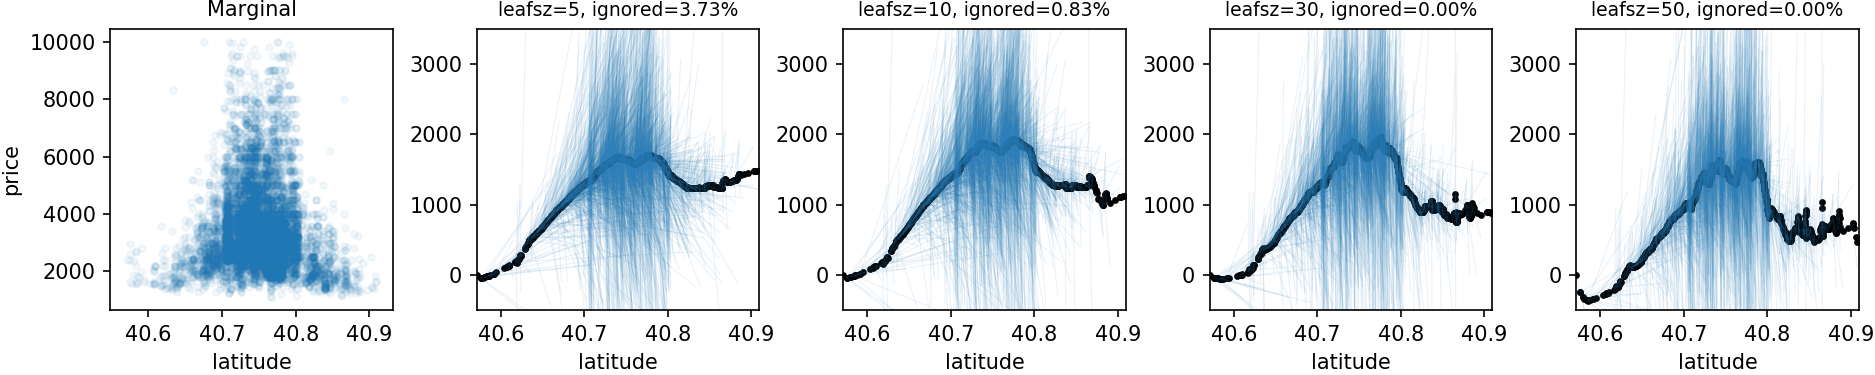
\includegraphics[scale=0.5]{images/latitude_meta.png}
\caption{Hyper parameter grid for rent data showing latitude versus price; 10,000 observations.}
\label{fig:latitude_grid}
\end{center}
\end{figure}

\figref{fig:bath_grid} shows the results of {\tt plot\_stratpd\_gridsearch()} operating on $x_{\it bathrooms}$ versus rent price. The partial dependence curve is stable, which again provides confidence in that partial dependence relationship.

\begin{figure}[htbp]
\begin{center}
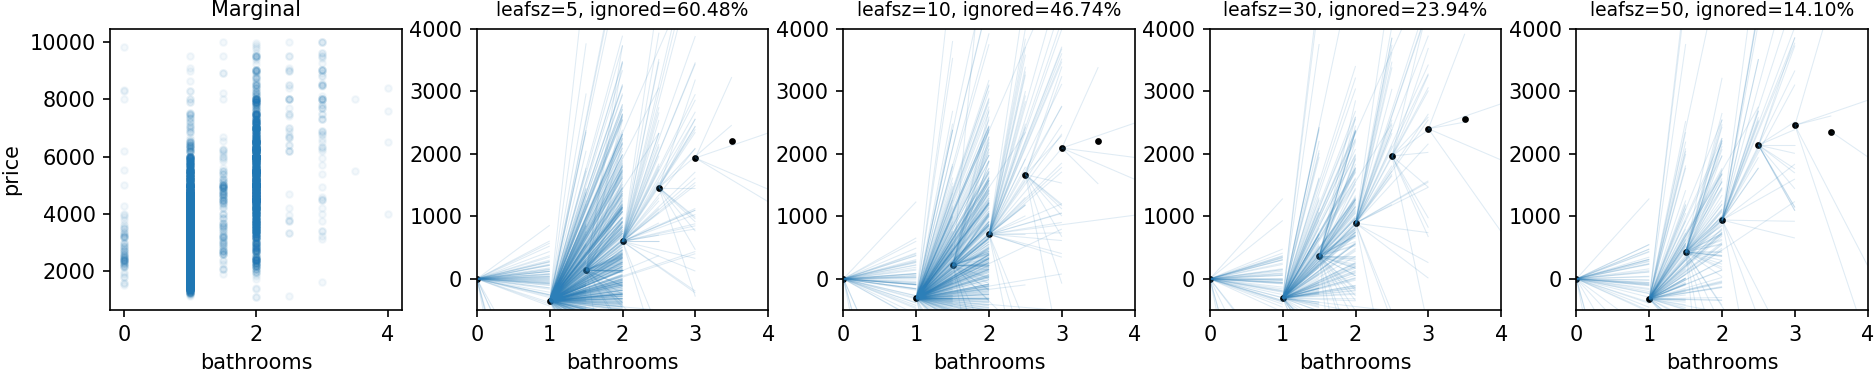
\includegraphics[scale=0.5]{images/bathrooms_meta.png}
\caption{Hyper parameter grid for apartment rent data showing bathrooms versus price; 10,000 observations.}
\label{fig:bath_grid}
\end{center}
\end{figure}

\cspd{} also uses hyper parameter {\it min\_samples\_leaf} and \figref{fig:weather_grid} shows $x_{\it state}$ versus temperature for the weather data set across multiple {\it min\_samples\_leaf} values.  The graphs show that when the leaf sizes too small, \cspd{} underestimates the effect of $x_{\it state}$ on temperature. Choosing a {\it min\_samples\_leaf} (2) that is less than the number of categories (4) means that \cspd{} cannot consider the relationship of all categories at once. After {\it min\_samples\_leaf}=20, \cspd{} finds the appropriate categorical partial dependence and holds study.

\begin{figure}[htbp]
\begin{center}
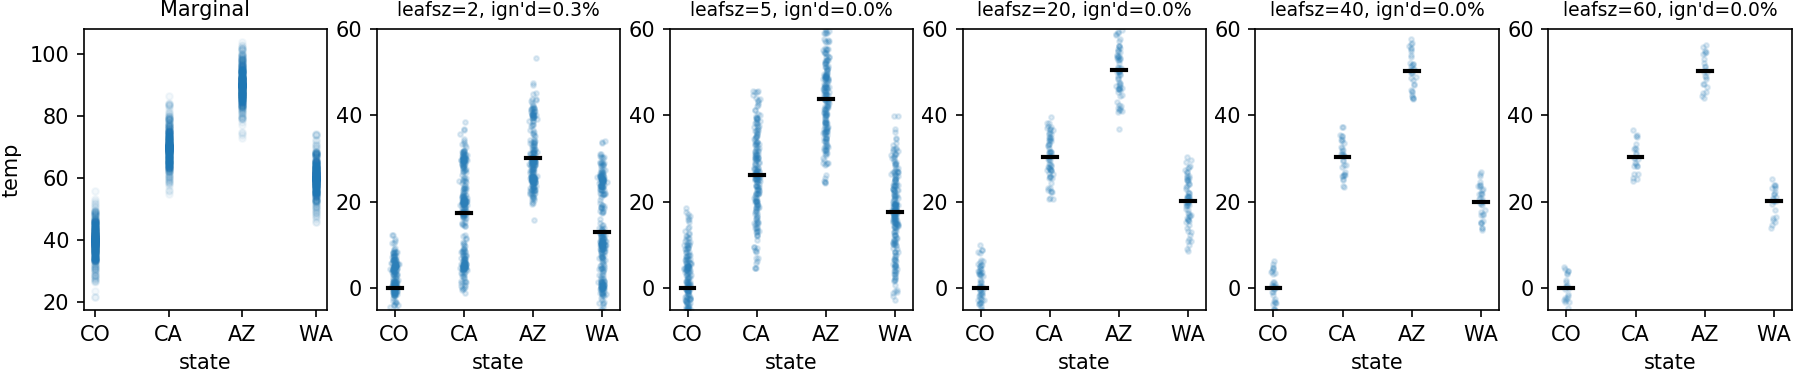
\includegraphics[scale=0.55]{images/state_temp_meta.png}
\caption{Hyper parameter grid for weather data using Equation \eqref{eq:weather} showing categorical variable state versus price.  A minimum of 20 samples per leaf is required to get an accurate plot.}
\label{fig:weather_grid}
\end{center}
\end{figure}


As discussed in \secref{sec:dup}, multiple trees are useful for dealing with duplicate columns in our experience. To engage random forest functionality, rather than simple decision tree \xnc{} partitioning, there are three more hyper parameters:

\begin{enumerate}
\item {\it ntrees}. The number of trees in the random forest. The default is 1; i.e., a decision tree.
\item {\it max\_features}. The number of features considered by the random forest when partitioning feature space. Decision trees use a default of 1.0, meaning consider all features, but random forests typically use $sqrt(p)$ or similar.
\item {\it bootstrap}.  Sample \xnc{} to get $n$ observations with replacement. Decision trees use a default of false, so this must be set to true to get a random forest.
\end{enumerate}

\section{Discussion and Future Work}

In this paper, we present an approach to partial dependence that addresses the issues encountered by other solutions.  Linear regression models are not always powerful enough and cannot be used when $p>n$; PD and ICE plots are biased in the presence of codependent variables (see \figref{fig:height_vs_weight}, \figref{fig:education_vs_weight}) and yield sometimes radically different results for the same data set, depending on the model chosen by the user (see \figref{fig:baths_price}, \figref{fig:4var}).

The \spd{}  approach is to stratify a data set into groups of observations that are similar in \xnc{} through the use of a decision tree or random forest. Any fluctuations of $y$ within a group (leaf) are most likely due to $x_c$, which lets us consider just $x_c$'s effect on $y$ while holding \xnc{} constant. We characterize the relationship of $x_c$ to $y$ within a group by fitting linear models through the unique $x_c$ values of that leaf.  To combine the resulting coefficients across the entire $x_c$ space and across leaves, \spd{} takes the weighted average of all coefficients that overlap region $R$ of the full $x_c$ space; in our implementation, the $R$ regions are taken to be the unique $x_c$ values. The combined slope coefficients give an overall approximation to the partial derivative of $y$ with respect to $x_c$ and the numerical integration gives the partial dependence plot. Categorical variables are handled with a different but similar algorithm that groups $y$ by $x_c$ category, computes the average $y$ for each category, and subtracts the overall average of $y$ in that leaf to strip away contributions from \xnc. We provide algorithms for numerical and categorical data in \appdxref{appendix:algorithms} and Python 3 source code at {\small \url{https://github.com/parrt/stratx}}.

The most important advantage of \spd{} is that it directly characterizes the relationship between $y$ and $x_c$ \emph{without} without relying on a user's fallible model. In this way \spd{} is {\em model independent}, rather than {\em model agnostic}, meaning that it will characterize marginal relationships the same way no matter the user's choice of machine learning algorithm.  While \spd{} trains a decision tree internally, the algorithm does so merely to partition feature space, never to make predictions with the tree. Surprisingly, \spd{} does not even need $y$ to  partition \xnc{} space, as we demonstrated in \secref{sec:partitioning} (see \figref{fig:rent_weight_unsup}), which strengthens our claim of model independence. 

Another advantage over previous techniques is that \spd{} isolates the contribution of $x_c$ to $y$ well, at least on the data sets we've tested, even in the presence of highly-codependent variables. This is true for the synthetic data sets, where we know the answer, and for two real data sets: NYC apartment rent prices and bulldozer sales. The rent and bulldozer plots are plausible and, moreover, are much more likely than those given by PD and ICE (see \figref{fig:baths_price}, \figref{fig:bulldozer}).  The results from PD and ICE are questionable anyway because different $\widehat{f}(X)$ models on the same data sets give very different results.

Our approach has just one primary hyper parameter, {\it min\_samples\_leaf}, the minimum leaf size to use during decision tree construction. (To engage the random forest functionality, there are other hyper parameters per \secref{sec:tuning}.) Our default for {\it min\_samples\_leaf} is 10 observations per leaf and the minimum {\it min\_samples\_leaf} is two in order to fit a localized linear model.  Generally speaking, larger leaf sizes are desirable because they are able to capture more nonlinearities and are less susceptible to noise.  As the leaf size grows, however, one risks introducing contributions from \xnc{} into the relationship between $x_c$ and $y$. We recommend examining the plots  for multiple values of {\it min\_samples\_leaf}. The more consistent the plot across {\it min\_samples\_leaf} values, the higher the confidence we have in the results. For example, we provided evidence of stability in the hyper parameter with \figref{fig:latitude_grid}, \figref{fig:bath_grid}, \figref{fig:weather_grid}. 

Experience applying \spd{} suggests two limitations. First, \spd{} can only hold constant variables included in the $\bf X$ matrix presented to it, but of course this is true for any partial dependence method. For example, \figref{fig:bulldozer} is likely biased towards a traditional marginal plot than is necessary, because we included only three codependent features in $\bf X$ for demonstration purposes.  

Second, \spd{} appears to be more sensitive to noisy variables than PD and ICE, at least for the low signal-to-noise ratios found in Equation \eqref{eq:bigX} and Equation \eqref{eq:parabola}. PD and ICE have a distinct advantage because they make use of a fitted model, $\widehat{f}(X)$.  Consider that PD and ICE plots derived from linear $\widehat{f}(X)$ models are restricted to lines, which gives them an advantage if the underlying relationship is linear. Of course, the true $f(X)$ relationship is unknown and so choosing the right model is critical. Even nonparametric models, such as random forests, have a predetermined fit (``shape'') for $x_c$ versus $y$. For $x_c=x_1$ in Equation \eqref{eq:parabola}, a random forest $\widehat{f}(X)$ will perforce generate (albeit stairstepped) parabola-like curves as PD and ICE algorithms shift $x_1$ through range $[-1,1]$. We did not observe problems with \spd{{} for the real data sets, which definitely have noise, but a much higher signal-to-noise ratio than the noisy synthetic data sets.  As opposed to noisy predictive variables, adding superfluous noise variables does not confuse or change the \spd{} plot.  This is true for PD and ICE as well, as long as the user chooses a model, such as random forests, that ignore  superfluous variables. A word of caution concerning \spd{} plots. While \spd{} identifies relationships in known synthetic data sets and gives plausible results that are stable in the hyper parameter for real data sets, small fluctuations in the plots are generally not meaningful. Look for the overall trend and shape of the curve.

The next step in our research is clearly to extend \spd{} to classifiers, as we have only addressed regressors so far.  Along the lines suggested by \cite{PDP}, a promising approach to partial dependence for classifiers would be to swap out \spd{}'s localized linear regression models for localized logistic regression (one-versus-rest) models.


\begin{appendices}

\section{CatStratPD for categorical variables}\label{appendix:catstrat}

The stratification approach can also capture how a categorical variable $x_c$ affects $y$, instead of just a single category at a time (if one were forced to dummy-encode $x_c$). As with \spd{},  \cspd{} (Algorithm 2) stratifies $\bf X$ into groups of similar \xnc{} features by training a decision tree regressor on $({\bf X}, {\bf y})$, yielding a collection of leaves. But, because categorical variables can be unordered nominal variables, the notion of $y$ slope is not meaningful between two categories.  Instead, the partial dependence plot for categorical variables shows how each category differs on average from the other categories. The category differences can be plotted as zero-centered deltas or shifted up so the lowest delta is zero.

For simplicity, we will write $(x^{(L)}, y^{(L)})$ as shorthand for the collection $\{(x_ic, y_i)\}_{i \in L}$ going forward. \cspd{} groups leaf observations $(x^{(L)}, y^{(L)})$ by the categories in $x^{(L)}$ and computes the average $y^{(L)}$ value per category $k$. To erase the $y$-contributions of \xnc{}, \cspd{} subtracts the average of $y^{(L)}$ from all leaf category averages, yielding a zero-centered relative increase or decrease in $y$ for each category:\\

\noindent ${\bf y}^{(L,k)} = y^{(L)}[x^{(L)}=k]$~~~~~~~~~~~~~({\it Group leaf $x_c$ by category $k$})\\
$n^{(L,k)} = |{\bf y}^{(L,k)}|$ if $|unique(x^{(L)})| > 1$ else 0\\
$\overline{y}^{(L,k)} = \frac{1}{n^{(L,k)}} \Sigma_{i=1}^{n^{(L,k)}} y_i^{(L,k)}$ ~~~~~~~~({\it Mean of leaf $y^{(L)}$ for category $k$})\\
$\Delta^{(L,k)} = \overline{y}^{(L,k)} - \overline{y}^{(L)}$ ~~~~~~~~~~~~~({\it Remove contribution of $x_{\overline{c}}$ to $y^{(L)}$})\\

\noindent Then, to get the overall contribution of $x_c$ to $y$ for category $k$, \cspd{} computes the weighted average of the leaf contributions for $k$ from all $L$:\\

\noindent $n^{(k)} = \Sigma_{T \in {\it rf}} \Sigma_{L \in T} ~n^{(L,k)}$~\,~~~~~~~~~~~~~~~({\it Num supporting observations for $k$})\\
$\Delta^{(k)} = \frac{1}{n^{(k)}} \Sigma_{T \in {\it rf}} \Sigma_{L \in T} \,n^{(L,k)}\Delta^{(L,k)}$~~~~({\it Delta for $k$ is weighted average across leaves})\\

\noindent Subtracting the \xnc{} contribution, $\overline{y}^{(L)}$, normalizes all $\Delta^{(L,k)}$ so they are relative to 0, providing a common baseline from which to average contributions across leaves. When there is only one category in $L$, the leaf does not support any conclusions about changes in $y$ for any category so $n^{(L,k)}=0$, dropping it from the weighted average. 

Plotting category $k$ against $\Delta^{(k)}$ gives a zero-centered partial dependence plot. The {\tt stratx} package shifts all $\Delta^{(k)}$ so the minimum $\Delta^{(k)}$ is 0 as we find it easier to interpret the plots. Consider the synthetic weather data shown in \figref{fig:state_vs_temp}(a) where temperature varies in sinusoidal fashion over the year and with different baseline temperatures per state:

\begin{equation}\label{eq:weather}
y = t[x_{\it state}] + sin(\frac{2 \pi}{365} x_{\it dayofyear} + \frac{365}{2}) \times \epsilon, ~~~ \epsilon \sim N(\mu=-5,\sigma=5)
\end{equation}

\noindent where the baseline $t$ per state is $\{{\it CA}=70, {\it CO}=40, {\it AZ}=90, {\it WA}=60\}$. Each sinusoid in \figref{fig:state_vs_temp}(a) is the average of three years' temperature data.

The categorical partial dependence plot for $x_{\it state}$ is shown in \figref{fig:state_vs_temp}(b).
\cspd{} stratifies \xnc{}=$\{x_{\it dayofyear}, x_{\it year}\}$ then groups these similar time buckets (leaves) by $x_{\it state}$ and computes the average temperature per state in $L$. For each $L$, the average temperature in $L$ is subtracted from the average temperature per state in $L$ to get deltas, which are represented by blue dots in \figref{fig:state_vs_temp}(b). The overall temperature estimate per state is the average of those leaf averages, represented by a solid black dash. We use a strip plot to exhibit the variation and density of $y$ values per category. The \cspd{} plot accurately identifies the baseline temperature per state, as does the PD/ICE plot in \figref{fig:state_vs_temp}(c).

\begin{figure}[htbp]
\begin{center}
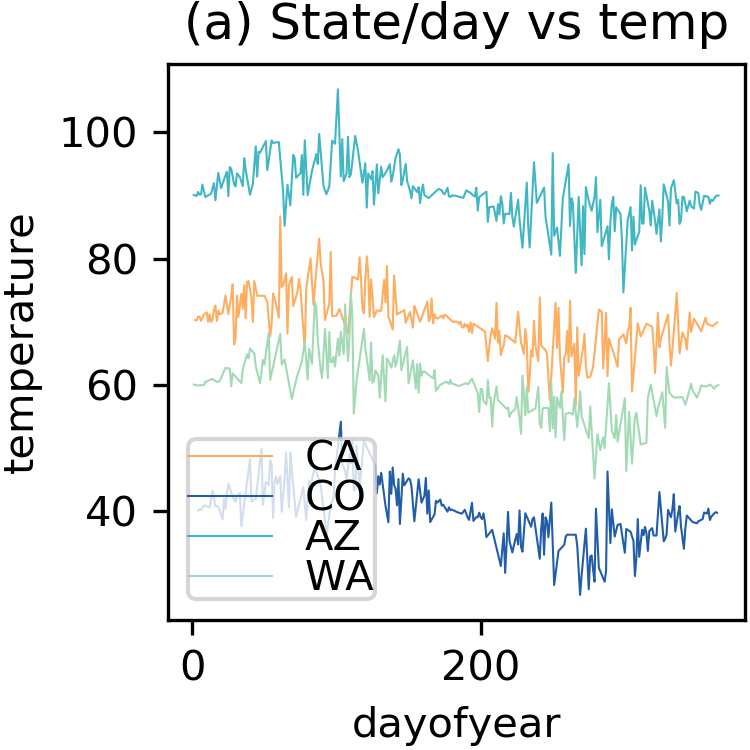
\includegraphics[scale=0.7]{images/dayofyear_vs_temp.png}
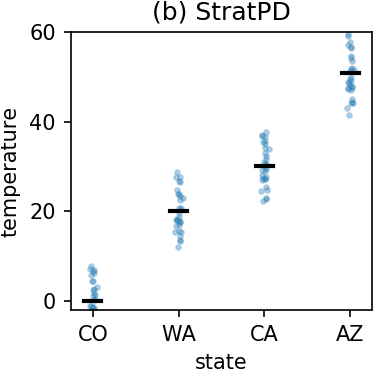
\includegraphics[scale=0.7]{images/state_vs_temp_stratpd.png}
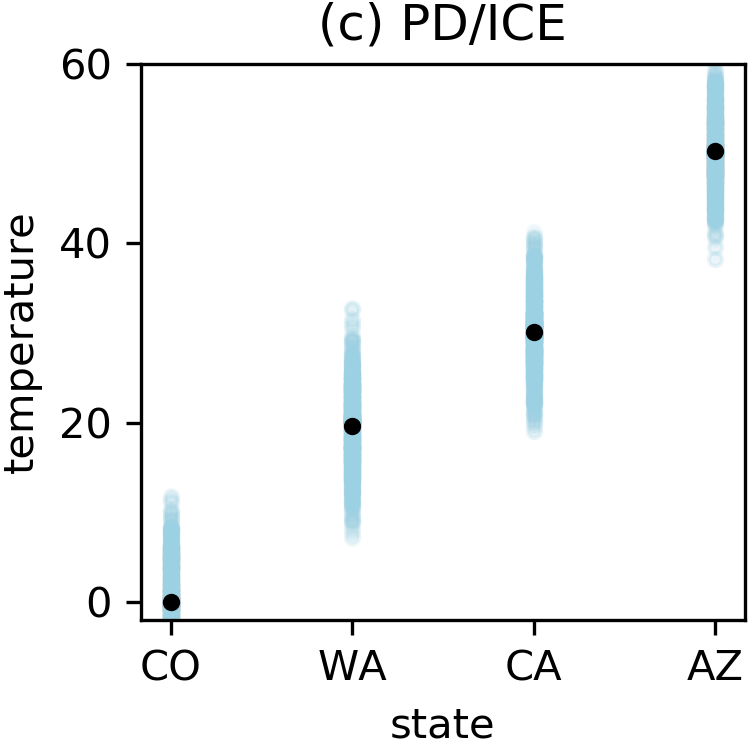
\includegraphics[scale=0.7]{images/state_vs_temp_pdp.png}
\caption{Plots from synthetic data from Equation \eqref{eq:weather} for categorical $x_c$ variables: (a) marginal plot of dayofyear versus temperature for four US states, (b) \spd{} plot, and (c) PD/ICE plot. Both \spd{} and PD/ICE capture the appropriate relationship, given the lack of codependence between state and other variables.}
\label{fig:state_vs_temp}
\end{center}
\end{figure}

\newpage
\section{Algorithms}\label{appendix:algorithms}

\setlength{\algomargin}{5pt}
\begin{algorithm}[]
\DontPrintSemicolon
\LinesNumbered
\SetAlgorithmName{Algorithm}{List of Algorithms}
\SetAlgoSkip{}
\SetInd{.5em}{.5em}
\TitleOfAlgo{{\em StratPD}}
\small
\KwIn{$\begin{array}[t]{l}
{\bf X}, {\bf y}, c,\\
{\it ntrees=1}, {\it bootstrap=false}, {\it max\_split\_features=all},\\
{\it min\_samples\_leaf}, {\it nbins}\\
\end{array}$
}
\KwOut{collection of $\beta_R$ coefficients across $x_c$, partial dependence curve}
Train random forest regressor $\it rf$ on (\xnc{}, $\bf y$) with hyper-parameters:\\
~~~~~$\it ntrees$, $\it bootstrap$, $\it max\_split\_features$, ${\it min\_samples\_leaf}$ \\
\ForEach{tree $T \in \it rf$}{
    \ForEach{leaf $L \in T$}{
    	$(x^{(L)}, y^{(L)})$ = $\{(x_{ic},  y_i)\}_{i \in L}$\\
	$uniqx^{(L)}$ = sorted(unique($x^{(L)}$))\\
	\If{$|uniqx^{(L)}| > 1$}{
		$bins$ = split $x^{(L)}$ into bins delimited by range $[uniqx^{(L)}_i,uniqx^{(L)}_{i+1}]$\\
    		\ForEach{bin $B \in bins$}{
    			$(x^{(B)}, y^{(B)})$ = $\{(x_{ic},  y_i)\}_{i \in B}$\\
    			$R^{(B)}$ = $[min(x^{(B)}), max(x^{(B)})]$\\
       	          	$n^{(B)} = |B|$\\
    		 	Fit linear model to $(B_x, B_y)$ giving $\beta_{B}$\\
	         }
	}
    }
}
$n = \Sigma_{T \in {\it rf}} \Sigma_{L \in T} \Sigma_{B \in L} n^{(B)}$~~~~~~~~~~~~~~~~~~~~~~~~~~~~({\it Num obs.'s supporting $\beta_B$ computations})\\
$uniqx$ = sorted(unique($x_c$))\\
\For{$i=1$ {\bf to} $|uniqx|-1$}{
	$R$ = $(uniqx_i, uniqx_{i+1})$\\
	\ForEach{bin $B$ created above}{
		$\beta_R = \frac{1}{n}\Sigma_{B \in R} \{ n^{(B)}\beta_{B} \}$
	}
}
$pd$ = numerically integrate $\beta_R$'s across $uniqx$\\
\Return{collection of all $\beta_R$, $pd$}
\label{alg:StratPD}
\end{algorithm}


\setlength{\algomargin}{5pt}
\begin{algorithm}[]
\DontPrintSemicolon
\LinesNumbered
\SetAlgorithmName{Algorithm}{List of Algorithms}
\SetAlgoSkip{}
\SetInd{.5em}{.5em}
\TitleOfAlgo{{\em CatStratPD}}
\small
\KwIn{$\begin{array}[t]{l}
{\bf X}, {\bf y}, c,\\
{\it ntrees=1}, {\it bootstrap=false}, {\it split\_features=all}, {\it min\_samples\_leaf}\\
\end{array}$
}
\KwOut{$\begin{array}[t]{l}
\Delta^{(k)} = \text{category } k \text{'s effect on } y \text{ where } mean(\Delta^{(k)})=0\\
n^{(k)} = \text{number of supported observations per category $k$}\\
\end{array}$
}
Train random forest regressor $\it rf$ on (\xnc{}, $\bf y$) with hyper-parameters:\\
~~~~~$\it ntrees$, $\it bootstrap$, $\it split\_features$, ${\it min\_samples\_leaf}$ \\
\ForEach{tree $T \in \it rf$}{
    \ForEach{leaf $L \in T$}{
        Let $(x^{(L)}, y^{(L)})$ = $\{(x_{ic},  y_i)\}_{i \in L}$\\
        Let $n_x^{(L)}=|unique(x^{(L)})|$\\
%        Let $K=\{k_1, k_2, \,\dots, k_{n_x}\}$ where \\
        ${\bf y}^{(L,k)} = y^{(L)}[x^{(L)}=k]$~~~~~~~~~~~~~({\it Group leaf $x_c$ by category $k$})\\
        $n^{(L,k)} = \begin{cases} |{\bf y}^{(L,k)}| &\mbox{if } n_x > 1 \\ 
        0 & otherwise\end{cases}$\\
        $\overline{y}^{(L,k)} = \frac{1}{|{\bf y}^{(L,k)}|} \Sigma_{i=1}^{|{\bf y}^{(L,k)}|} y_i^{(L,k)}$ ~~~~\,~({\it Mean of leaf $y^{(L)}$ for category $k$})\\
        $\Delta^{(L,k)} = \overline{y}^{(L,k)} - \overline{y}^{(L)}$ ~~~~~~~~~~~~~({\it Remove contribution of $x_{\overline{c}}$ to $y^{(L)}$})\\
    }
}
$n^{(k)} = \Sigma_{T \in {\it rf}} \Sigma_{L \in T} ~n^{(L,k)}$~~~~~~~~~~~~~~~~({\it Num supporting observations for $k$})\\
$\Delta^{(k)} = \frac{1}{n^{(k)}} \Sigma_{T \in {\it rf}} \Sigma_{L \in T} \,n^{(L,k)}\Delta^{(L,k)}$~~~~~~~({\it Delta for $k$ is weighted, averaged across leaves})\\
\Return{$\{{\Delta}^{(1)}, {\Delta}^{(2)}, \,\ldots, {\Delta}^{(k)}\}$, $\{{n}^{(1)}, {n}^{(2)}, \,\ldots, {n}^{(k)}\}$}\\
\label{alg:CatStratPD}
\end{algorithm}

\end{appendices}

\newpage
\bibliographystyle{apalike}

\bibliography{stratpd}
\end{document}